\chapter{光电倍增管的性能测试}
\label{ch:pmt_test}
由于制造工艺的限制,光电倍增管具有很强的个体差异性,即不同管子的性能差异较大。
因此,在光电倍增管大规模应用时,往往要求对每支管子进行详细的测试,以得到它们各自的性能参数信息。
利用这些信息,探测器的研制者可以淘汰性能参数不达标的管子,可以决定管子在探测器整体中的安装位置,可以得到管子的额定工作电压,甚至可以在探测器部署运行后调节其实际工作电压,最终使探测器整体的探测性能达到最佳。

对于PSD所使用的R4443型光电倍增管,Hamamatsu公司对每支出厂的管子进行了基本的性能测试(包括阳极暗电流、长时间稳定性、阴极/阳极的光灵敏度以及阴极/阳极的蓝光灵敏度),并提供了相应的测试结果。
然而,这些测试只在一个工作电压点进行,而且使用的测试条件(连续、强烈的白炽光照射)与R4443在PSD中的实际工作条件(低强度、低频率的脉冲光照射)迥异。
另外,PSD使用双打拿极引出的分压器电路与上述出厂测试使用的标准分压器差别较大,导致R4443的工作状态也不一致。
因此,这些参数信息只能定性地给出各支管子的基本性能,不能作为PSD研制过程的定量参考。

上述因素决定了:需要根据PSD的具体需求,在实验室独立对R4443光电倍增管进行性能参数测试。
为此,我们专门设计并搭建了一套的PMT批量测试平台。
本章对该测试平台进行了介绍,并详细叙述了该平台在R4443光电倍增管的性能测试中的应用以及测试结果。
根据测得的性能参数数据,依据性能最佳的原则,我们进一步对所有管子进行了筛选,选出了可以用于PSD安装的光电倍增管。

\section{PMT批量测试平台}
\label{sec:pmt_test:testbench}
PSD的研制过程中涉及大量的PMT测试工作,包括对570支R4443裸光电倍增管的细致性能测试以及在PSD建造过程中将近200个PMT组件的质量测试(详见第\ref{ch:construction}章)。
为了提高工作效率,减轻测试人员的工作负担,我们设计并建造了能够用于PMT大批量测试的专用测试平台。

\subsection{功能与特点}
\label{sec:pmt_test:testbench_functions}
PMT的批量测试是在大型探测器研制过程中经常碰到的工作。
因此,该测试平台虽然是为了DAMPE-PSD项目专门研制的,但我们在设计中充分考虑了该平台的拓展性和可移植性,使得它能够方便地应用于其它项目的PMT测试工作。
该测试平台的主要特点可以归结为如下几点:
\begin{enumerate}
	\item 测试容量大。大型探测器项目动辄涉及成百上千支PMT的测试,如果能够对多支PMT同时进行测试,就可以显著提高工作效率,加快项目进程。该测试平台最大测试容量达到25支PMT,满足大部分项目的测试需求。
	\item 自动化程度高。PMT的细致测试往往涉及不同的性能指标,一次完整的测试需要花费几个小时的时间。这个过程中,需要对大量的仪器设备进行重复操作,如升降高压、切换光强度、移动PMT位置等等。此时,人工操作不仅效率低,而且是不可靠的。因此,该测试平台的关键组件都是用了程控设备,并开发了相应的控制软件,实现了常用设备操的自动化。这样,在PMT的整个测试过程中,人工干预只存在于PMT的安装与卸载,以及相关软件的配置,提高了测试工作的可靠性。
	\item 功能完备。该测试平台能够满足很多潜在的测试需求,即便有些在PSD的研制过程中并不需要。因此,平台使用了一些特殊的硬件模块以及通用的仪器设备。尤其是,我们将三维移动性作为该平台的一个基本功能,使得平台可以用于PMT光阴极的位置扫描。
	\item 扩展性强。测试平台采用模块化设计,其硬件平台是可扩展的,各硬件模块之间的耦合相对松散。这方便了硬件的更换或升级,并可以实现较为复杂的测试方案。软件框架同样基于模块化设计,并对底层硬件进行了虚拟化,使得顶层的测试功能不因底层硬件的改动而有大的变动,增强了测试程序的可移植性。
\end{enumerate}

图\ref{fig:pmt_test:testbench_schematic}给出了PMT批量测试平台的原理框图。
该平台最多可以同时对25支PMT进行测试。光脉冲由一个蓝光LED产生,它经过积分球和集束光纤组成的光分配系统被分成25份,被分别传输到待测PMT的入射端面。
待测PMT都安置在一个固定平台上,而光源和光分配系统被固定在一个三维移动平台上。两个平台相对摆放,从而实现了对所有待测PMT的光阴极位置扫描。
固定平台上同时安置有两支监控PMT,也接受来自光分配系统的两路入射光脉冲。
在整个测试周期中,两支PMT的位置相对于入射光纤固定不变,因此它们被用于监控LED光源以及整个测试平台性能的稳定性。
这两个支撑平台以及上面的所有测试设备都被放置在一个大小为$176cm\times100cm\times78cm$的铝合金暗箱中(见图\ref{fig:pmt_test:blackbox}),箱子的内壁用黑色图层覆盖以降低内部的杂散光污染。

\begin{figure}[htb]
	\centering
	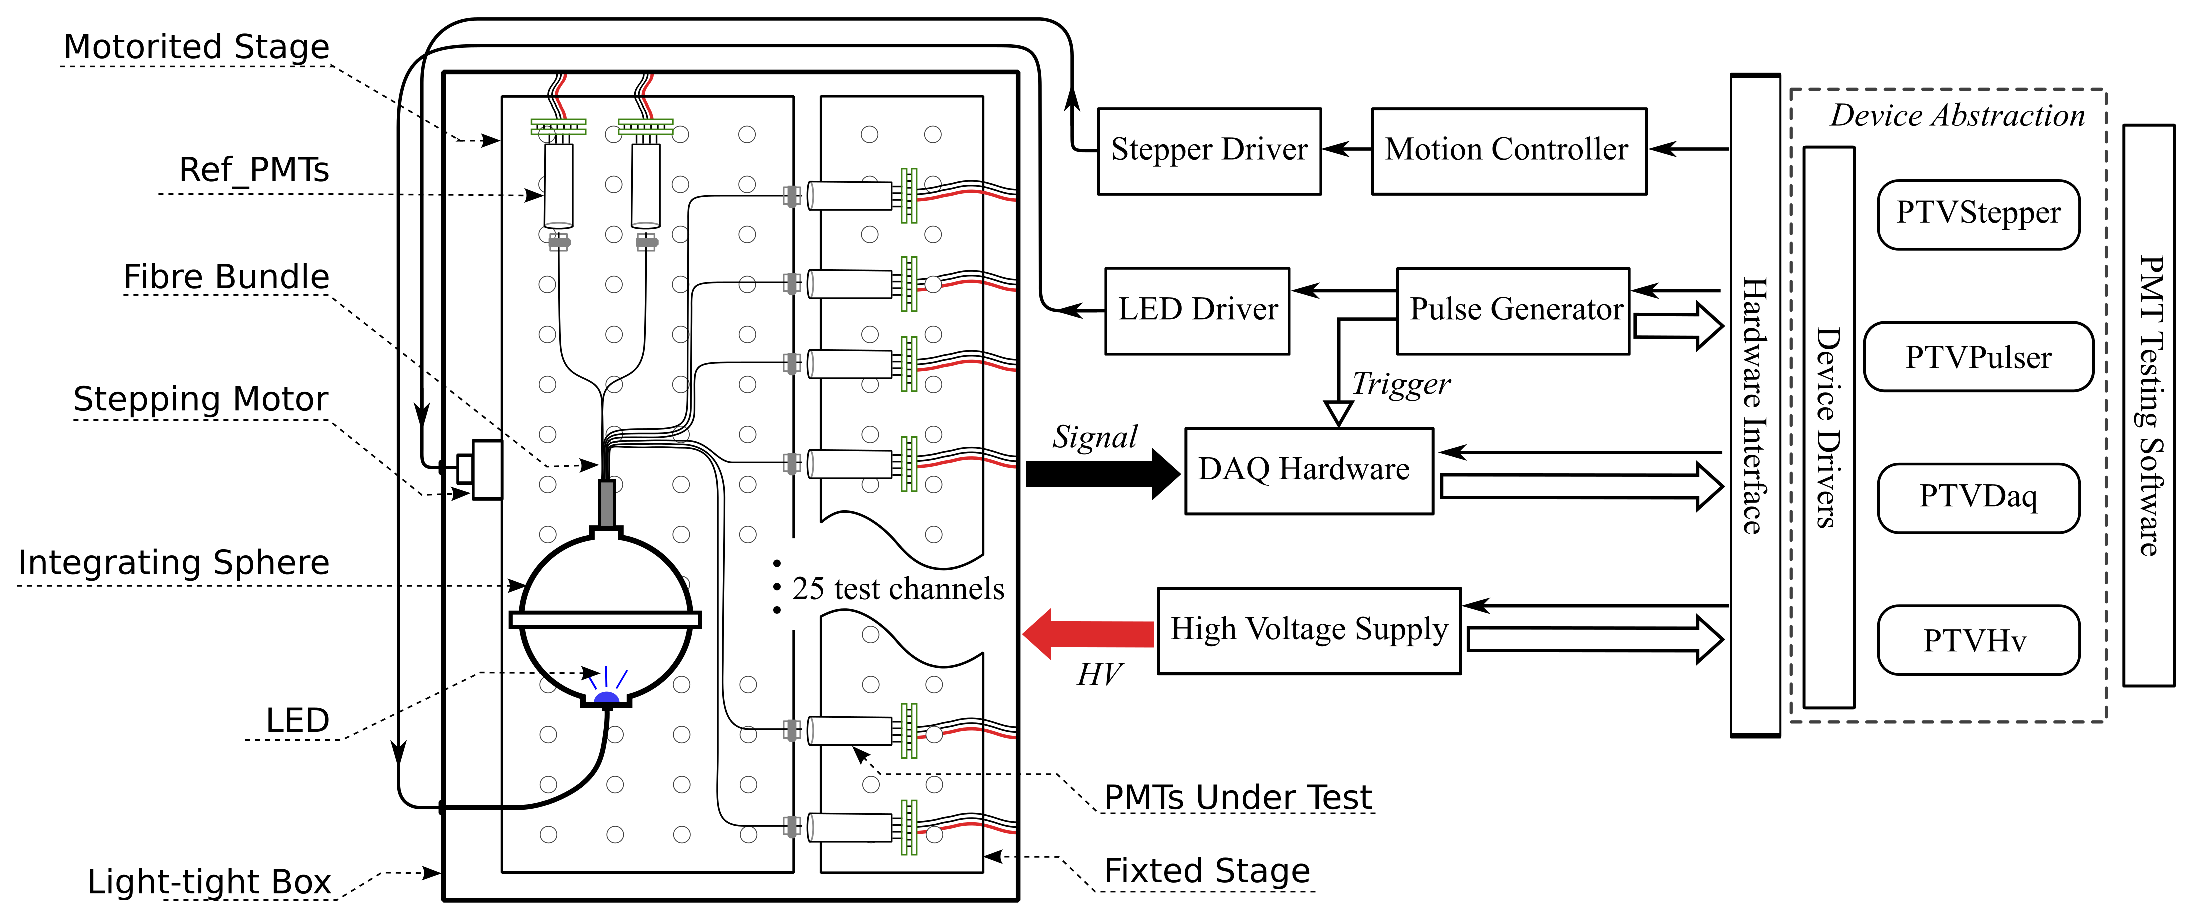
\includegraphics[width=\textwidth]{chap/pmt_test/fig/testbench_schematic.eps}
	\caption{PMT批量测试平台的原理框图}
	\label{fig:pmt_test:testbench_schematic}
\end{figure}

PMT测试平台的大部分辅助设备被都放置在铝合金暗箱的外围,它们与内部器件的连接线缆穿过箱子上不透光的通孔相互联接。
这些辅助设备可以被分为四个不同功能模块,分别为:运动控制模块,光脉冲驱动模块,数据获取模块(简称DAQ模块)以及高压供给模块。
运动控制模块和光驱动模块是和测试平台紧密联系在一起的,而与此相关的设备基本在所有的测试中都可以重复使用。
相反的,DAQ模块和高压供给模块与需要PMT测试的具体项目紧密联系,一般需要使用该项目定制的仪器设备进行测试。
作为一个通用的解决方案,我们为测试平台配备了一个基于CAMAC机箱的DAQ模块以及一个基于CAEN SY1527LC机箱\cite{sy1527lc}的高压供给模块。
这两个模块可以根据具体情况进行更换,在PSD的PMT性能测试中,我们就将上述CAMAC机箱替换成了PSD专用的地面检测系统(详见\ref{sec:pmt_test:characterization})。

最后,整个PMT测试平台系统被放置在一个十万级的洁净室中,室内温度被控制在$22\pm2$\si{\celsius}。

\subsection{硬件组成以及相关性能测试}
\label{sec:pmt_test:testbench_hardware}
% 总述硬件结构,之后依次介绍各组件以及相关测试结果。
% 主体平台
PMT测试平台的主体由一个固定平台和一个三维移动平台组成(见图\ref{fig:pmt_test:stages}),暗箱内的所有测试器件都被安置在它们上面。
\begin{figure}[htbp]
	\centering
	\subfloat[][铝合金暗箱]{
		\label{fig:pmt_test:blackbox}
		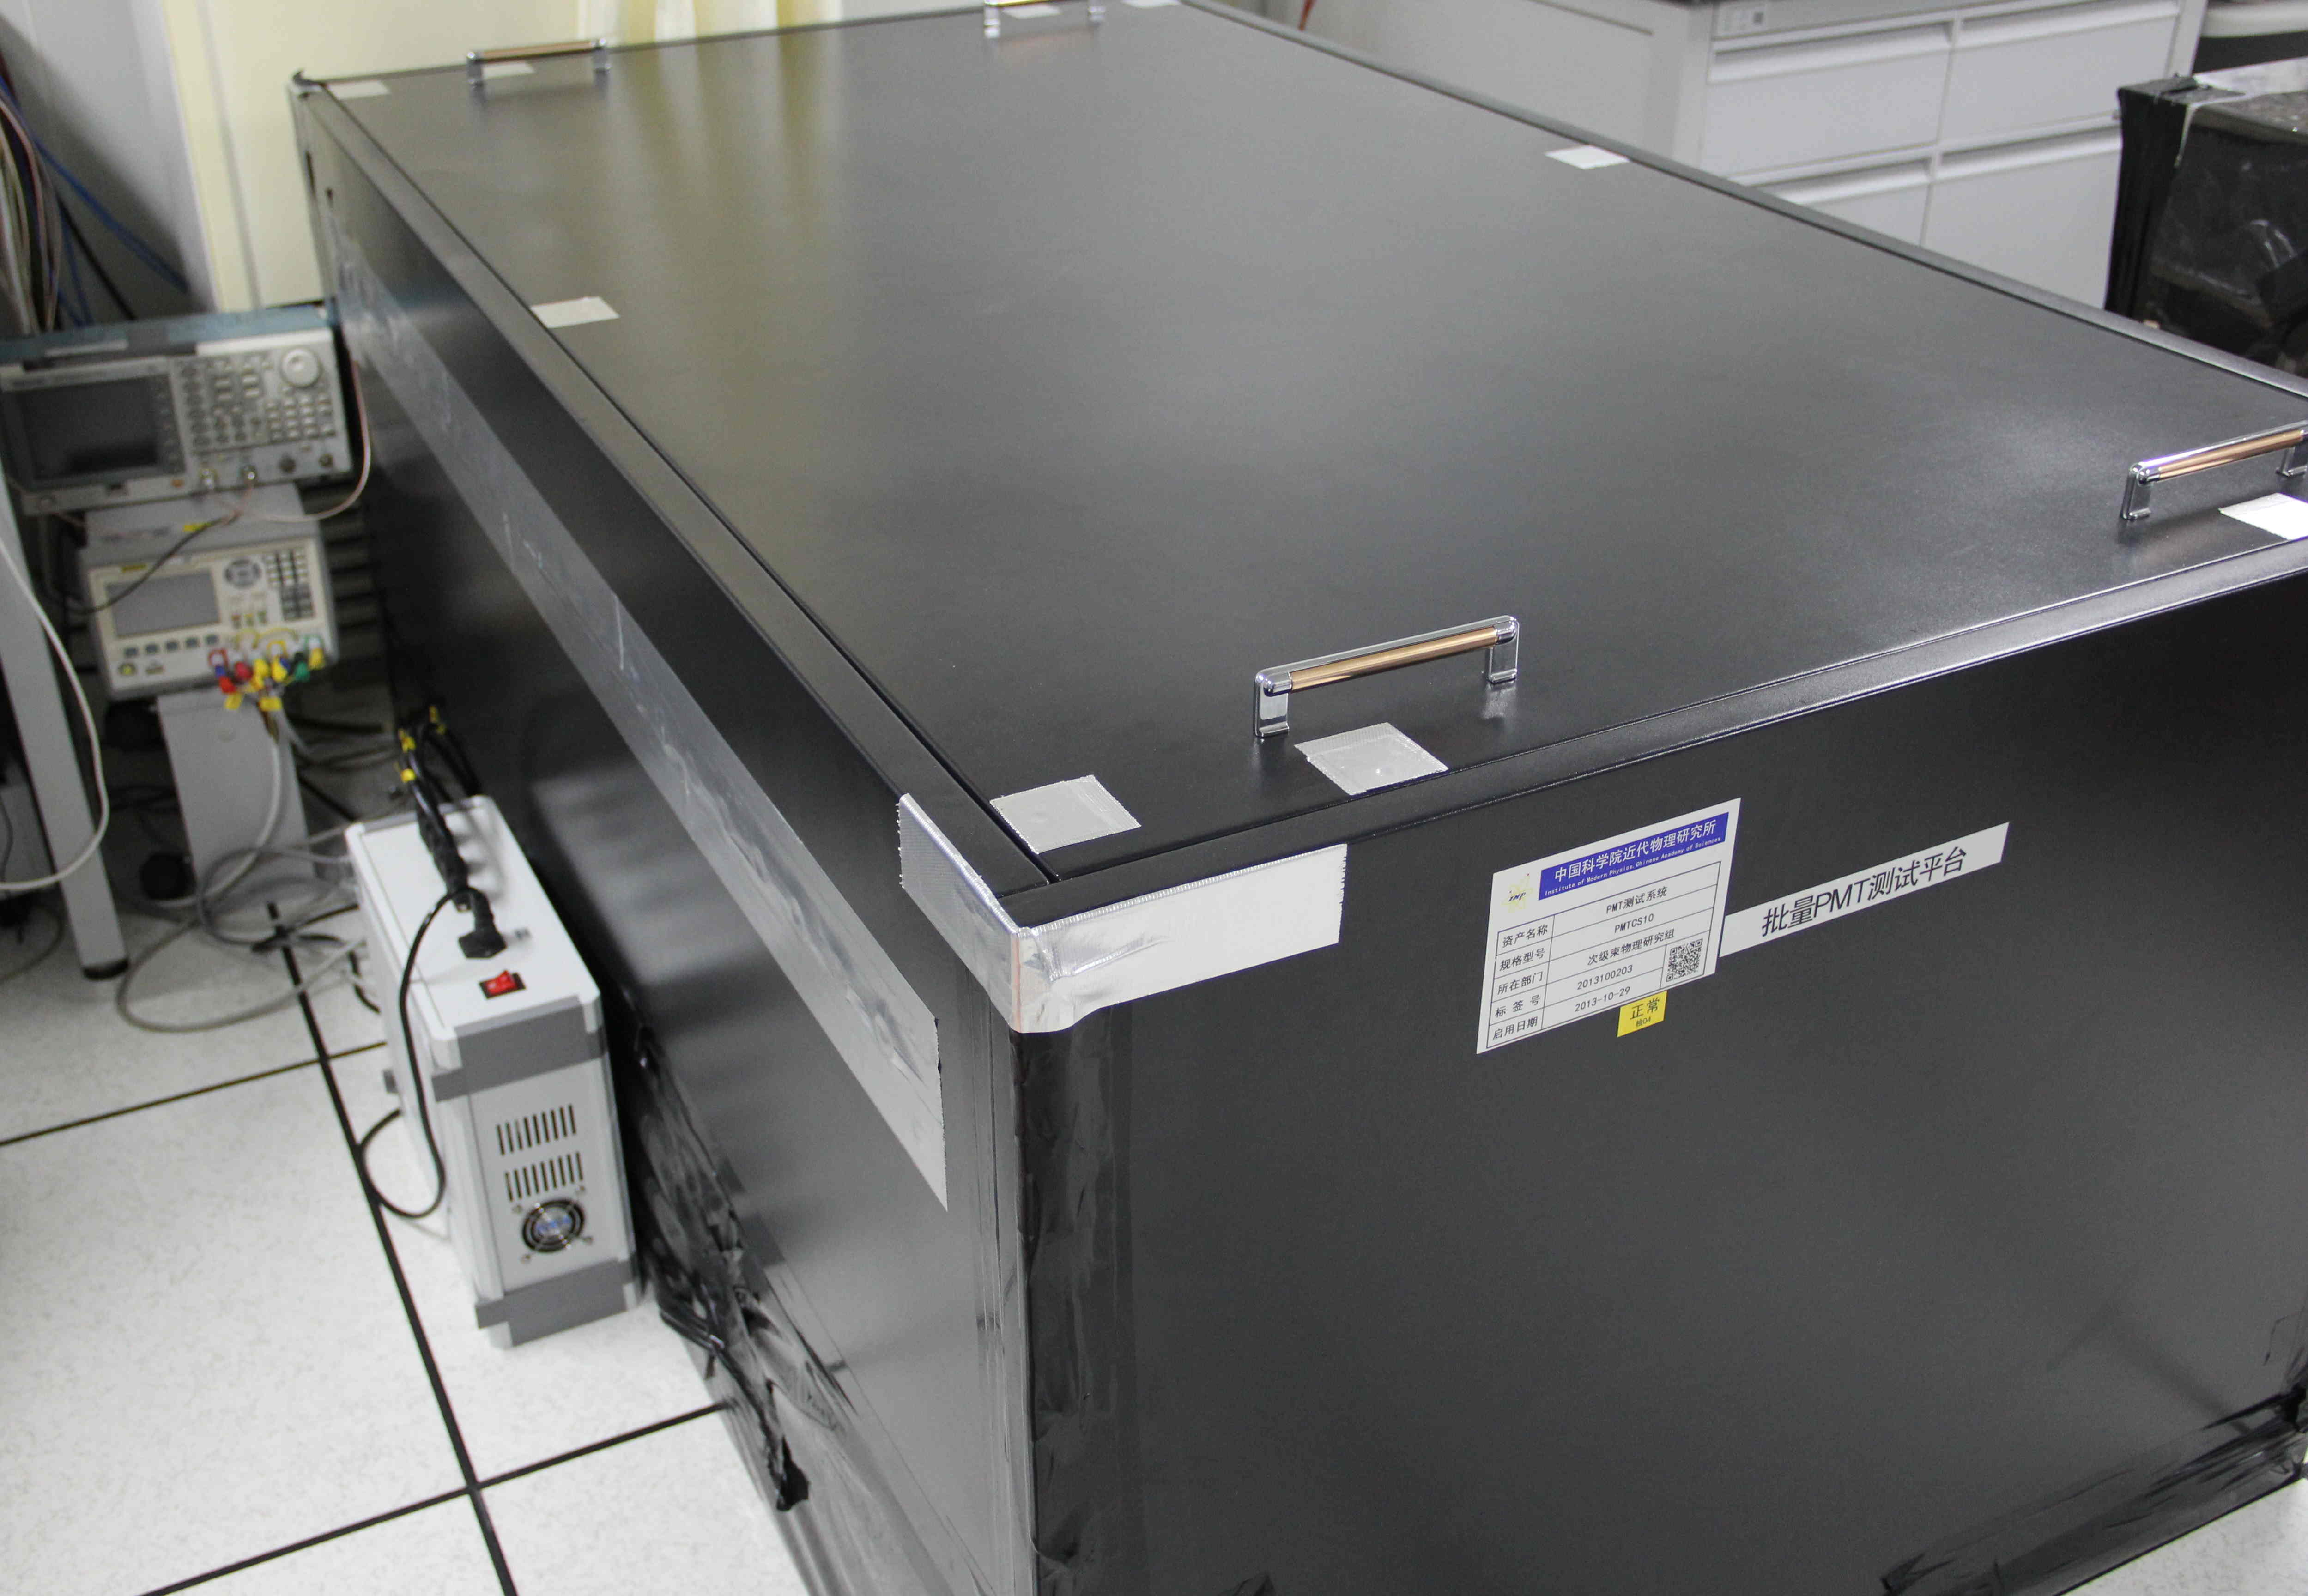
\includegraphics[width=0.49\textwidth]{chap/pmt_test/fig/black_box.jpg}
	}
	\subfloat[][三维移动平台与固定平台]{
		\label{fig:pmt_test:stages}
		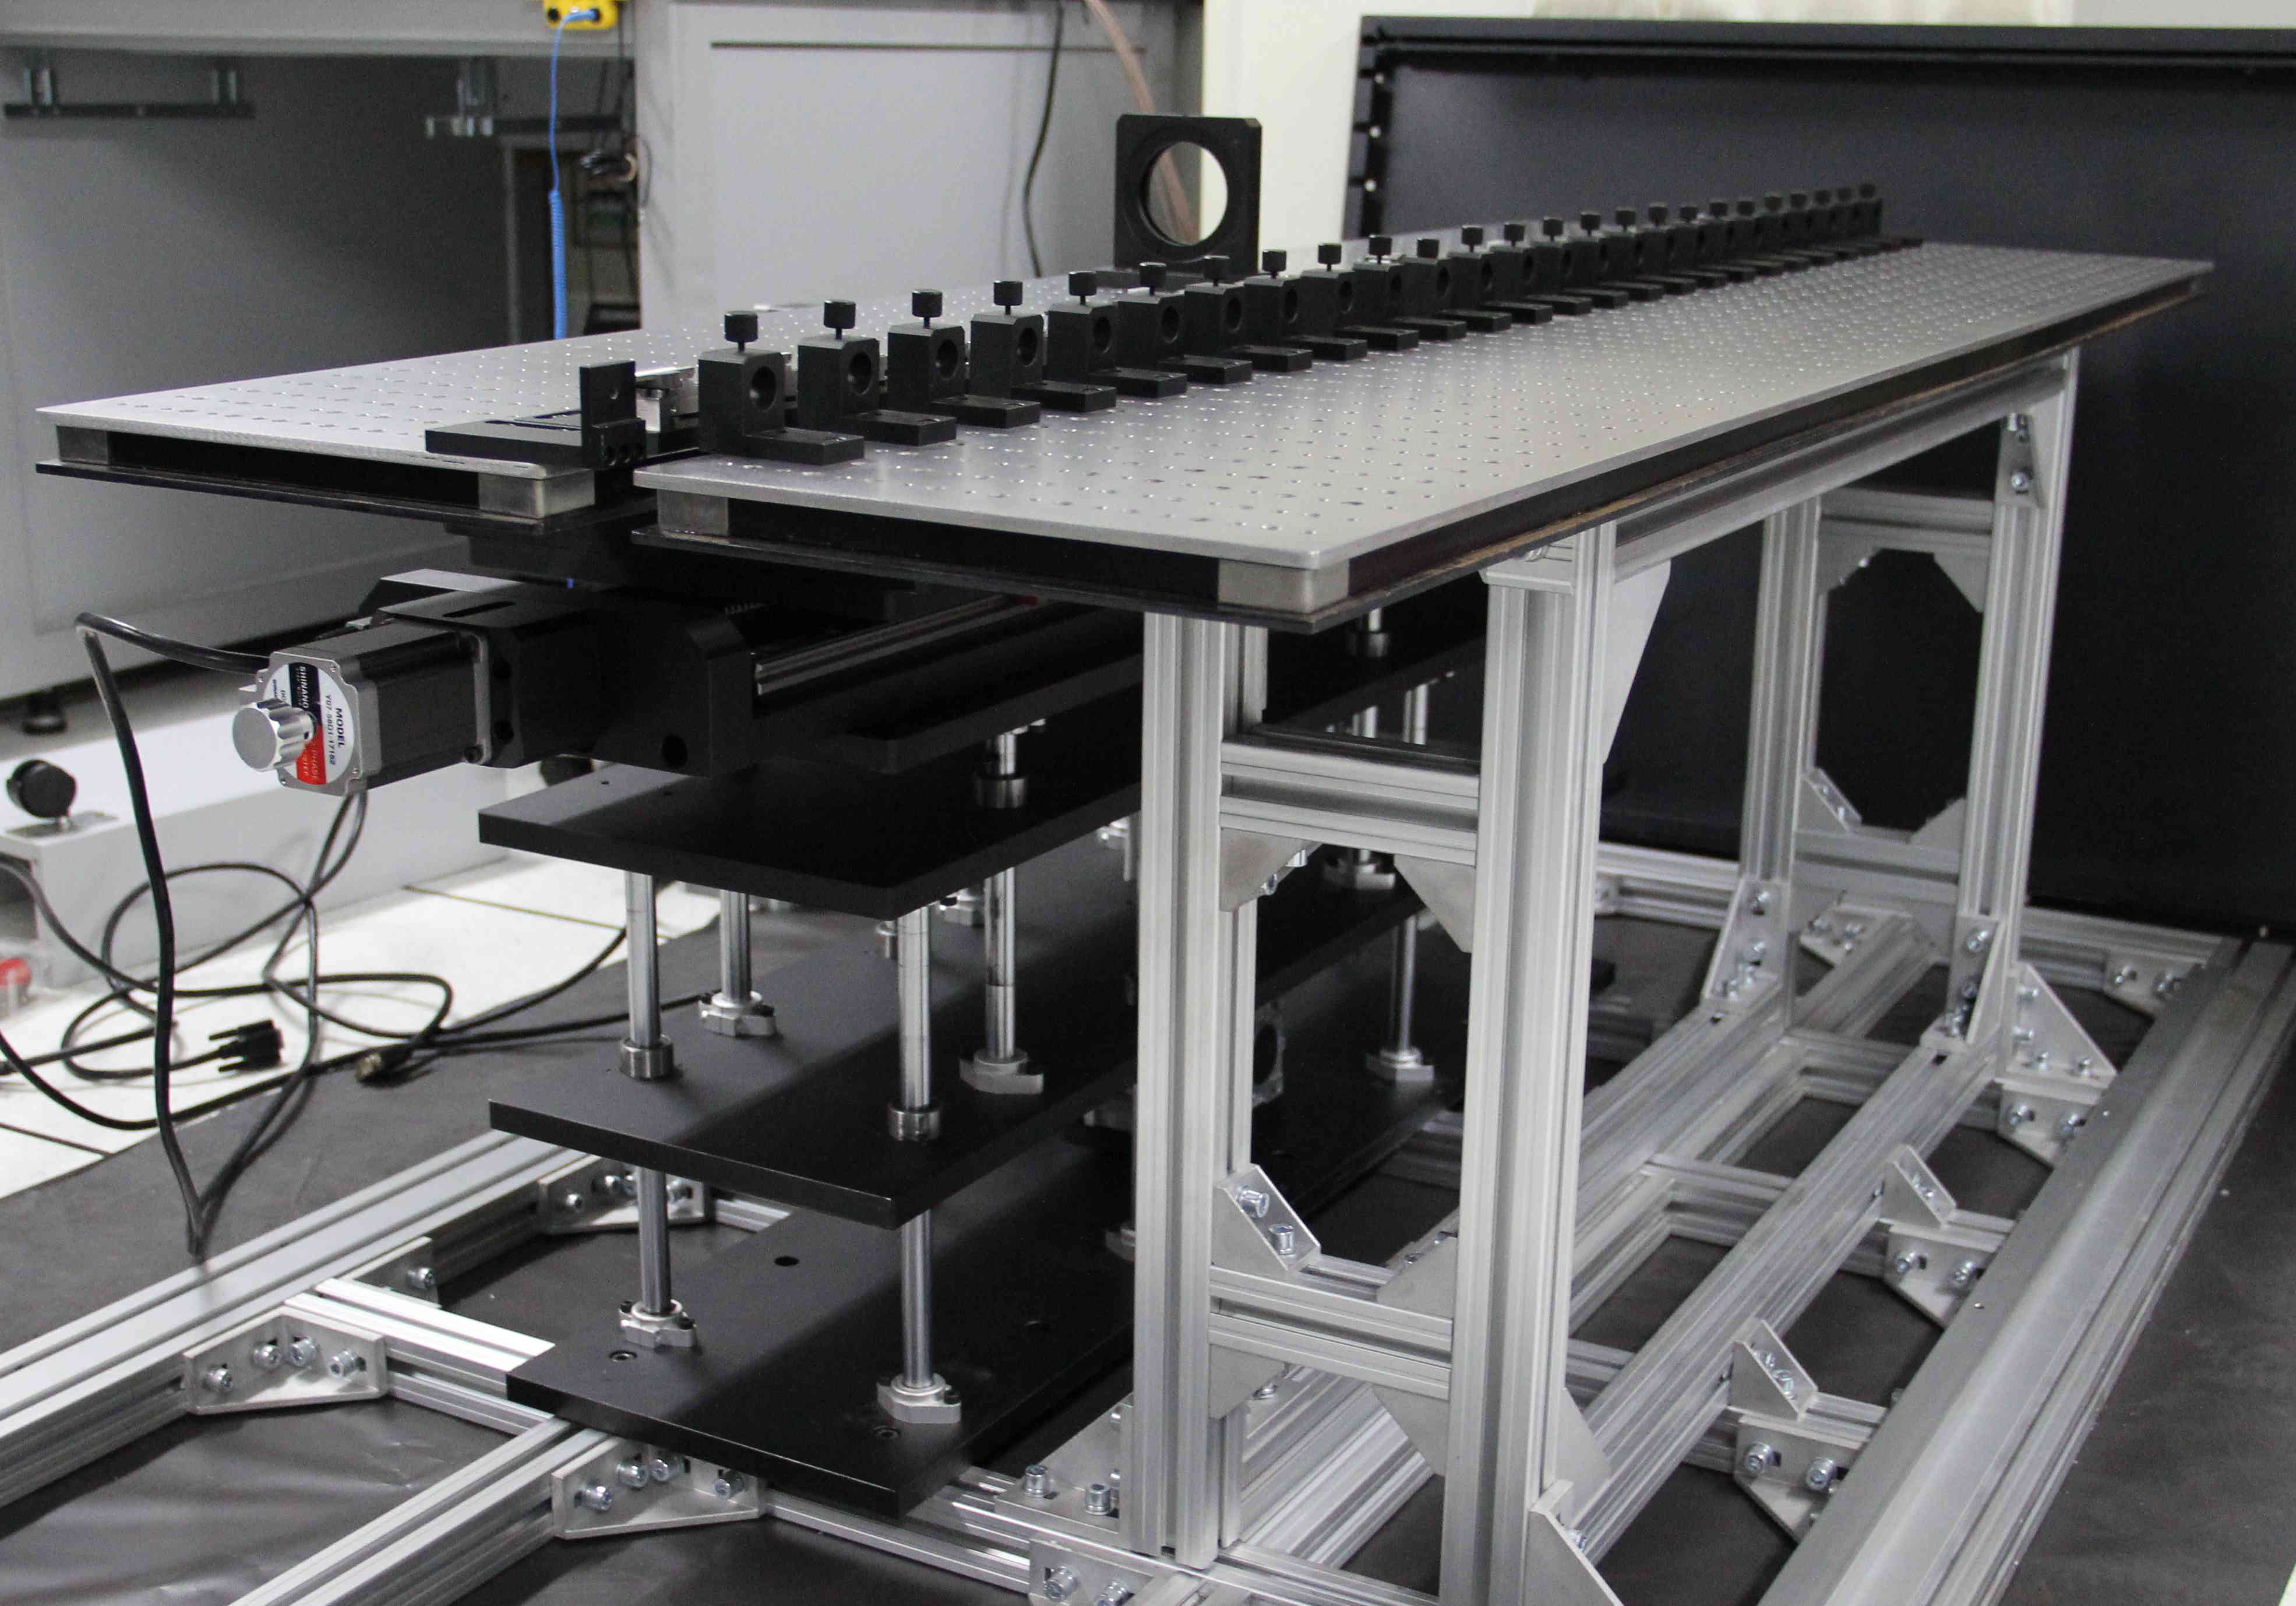
\includegraphics[width=0.49\textwidth]{chap/pmt_test/fig/stages.jpg}
	}
	\caption{PMT批量测试平台的主体结构}
	\label{fig:blindfigure}
\end{figure}
两个平台的台面各覆盖有一块面积为$1560mm\times250mm$的光学平板。
平板材质为\SI{2.5}{cm}厚度的不锈钢,因此可以有效抵抗重物放置带来的形变,保持台面上各器件位置的稳定性。
另外,光学平板上布满成网格排布的、并有M4和M6两种规格的螺纹孔,这不仅方便了台面上器件的安装与拆卸,并且提供了额外的摆放灵活性。
三维移动平台可以带动台面完成X-Y-Z三个方向的移动,每个方向都用一个步进电机驱动,其最大负载重量为\SI{30}{\kilo\gram}。
表\ref{tab:pmt_test:motorized_stage}列出了它的基本运动参数。
可以看到,平台的左右行程和上下行程使其能够对所有直径小于\SI{60}{\milli\meter}的PMT进行全面地光阴极扫描。
额外的第三维运动主要用于控制光纤与待测PMT之间的距离,在测试时尽量拉近光纤与PMT端面的距离,而在拆卸时拉远它们之间的距离,从而保护光纤不受意外损伤。
三个方向的步进电机都由一个运动控制器控制\cite{leetro},并可以利用PCI总线实现远程控制。
\begin{table}[htb]
	\centering	
	\begin{tabulary}{0.6\linewidth}{LC}
		\toprule[1.5pt]
		\textbf{项目} & \textbf{数值}	\\ 
		\midrule[1pt]
		最小步长		& \SI{1.56}{\micro\meter}	\\
		左右行程		& \SI{60}{\milli\meter}	\\
		上下行程		& \SI{70}{\milli\meter}	\\
		前后行程		& \SI{15}{\milli\meter}	\\
		\bottomrule[1.5pt]
	\end{tabulary}
	\caption{三维移动平台的基本运动参数}
	\label{tab:pmt_test:motorized_stage}	
\end{table}
为了方便操作和固定位置,我们还定制了专用的PMT夹具和光纤夹头,图\ref{fig:pmt_test:fixtures}展示了R4443和光纤固定在测试平台上的状态。
其中,光纤夹头可以实现水平方向上的微调,便于将光纤对准PMT光阴极中心(精度在\SI{0.5}{mm})。
% 紧固件
\begin{figure}[htbp]
	\centering
	\includegraphics[width=0.6\textwidth]{chap/pmt_test/fig/fixtures.jpg}
	\caption{PMT夹具和光纤夹头}
	\label{fig:pmt_test:fixtures}
\end{figure}

% 光源以及驱动
PMT测试系统使用大功率的蓝光LED(\SI{3}{\watt}, \SIrange{465}{485}{\nano\meter})作为光源。
该LED的发光光谱能够与大部分光阴极材料的光谱响应相吻合,而且曾被成功应用到HIRFL-RIBLL2外靶终端的中子墙光刻度系统中\cite{yuyuhong_led},其功率大小能够满足大量光通路的驱动要求。
为了使LED产生脉冲光,我们采用通用的脉冲发生器AFG3252\cite{afg3252}产生的方波信号来直接驱动LED发光。
虽然AFG3252不是专用的LED驱动器,但它的驱动效果能够满足我们的基本需求,如图\ref{fig:pmt_test:led_pulse}所示。
\begin{figure}[htbp]
	\centering
	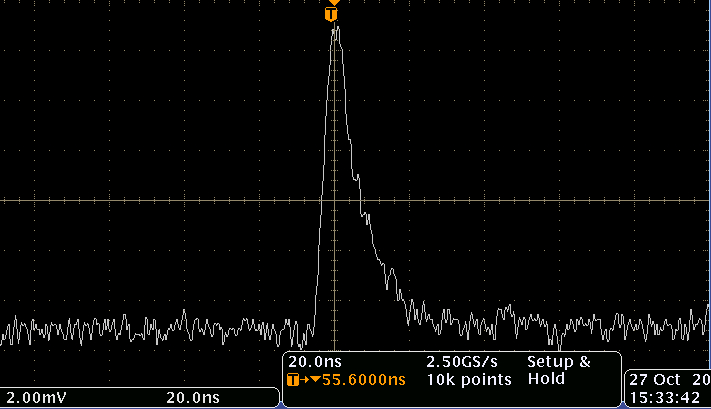
\includegraphics[width=0.65\textwidth]{chap/pmt_test/fig/led_pulse.jpg}
	\caption{\SI{30}{\nano\second}脉宽,\SI{5}{\nano\second}上升沿/下降沿的方波脉冲驱动LED发光得到的R4443输出波形}
	\label{fig:pmt_test:led_pulse}
\end{figure}
AFG3252的驱动脉冲参数可以在很大的范围内进行调整,而且精度很高,这是专用的LED驱动器达不到,因此可以满足各种各样的光输出要求,增强了PMT测试平台的通用性。
图\ref{fig:pmt_test:led_response}给出了不同脉宽、不同幅度的方波产生的LED光强变化,可以看到脉冲幅度与LED的输出光强并不成正比,这需要在使用中特别加以注意。
\begin{figure}[htbp]
	\centering
	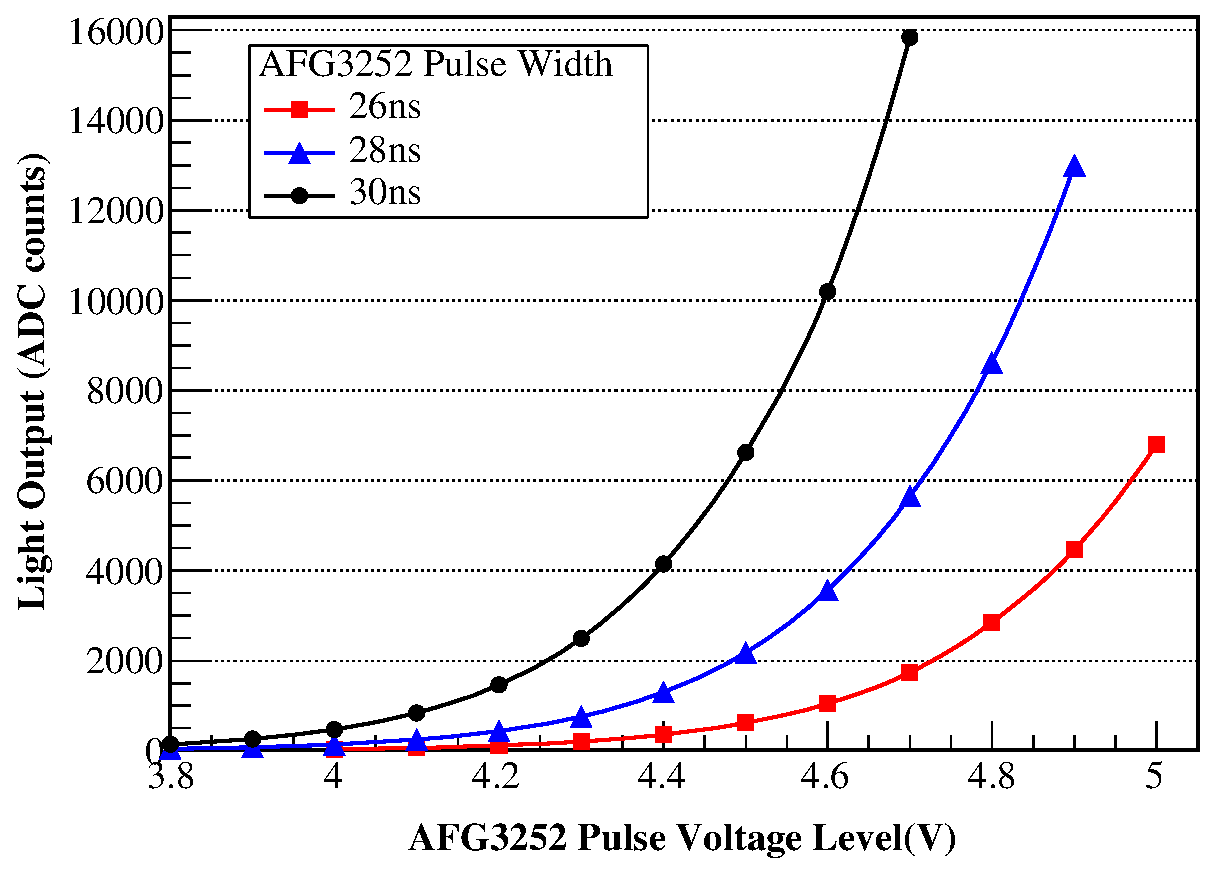
\includegraphics[width=0.7\textwidth]{chap/pmt_test/fig/led_response.eps}
	\caption{LED输出脉冲的光强度与AFG3253脉冲幅度的非线性关系}
	\label{fig:pmt_test:led_response}
\end{figure}
AFG3252的另外一个优点是:它的所有功能都可以在远程进行控制,而且接口丰富,我们可以选择熟悉的方式对其进行控制。
在PMT批量测试系统中,我们通过网口,并使用SCPI(Standard Commands for Programmable Instruments)命令\cite{afg3000_programmer_manual}对AFG3252进行远程操作。

% 积分球
LED发出的光脉冲通过集束光纤被分配到各支PMT,它与集束光纤之间通过一个\SI{5}{\centi\meter}的积分球耦合。LED、积分球和集束光纤一起构成了PMT测试系统的光分配系统,如图\ref{fig:pmt_test:light_distribution}。
其中LED通过导热硅胶固定在一个与积分球入射端口适配的底座上,而集束光纤通过三维位移台直接对准积分球出射端口的中心(参加见图\ref{fig:pmt_test:lightsource_integration})。
\begin{figure}[htbp]
	\centering
	\subfloat[][1)LED 2)积分球 3)集束光纤]{
		\label{fig:pmt_test:lightsource_components}
		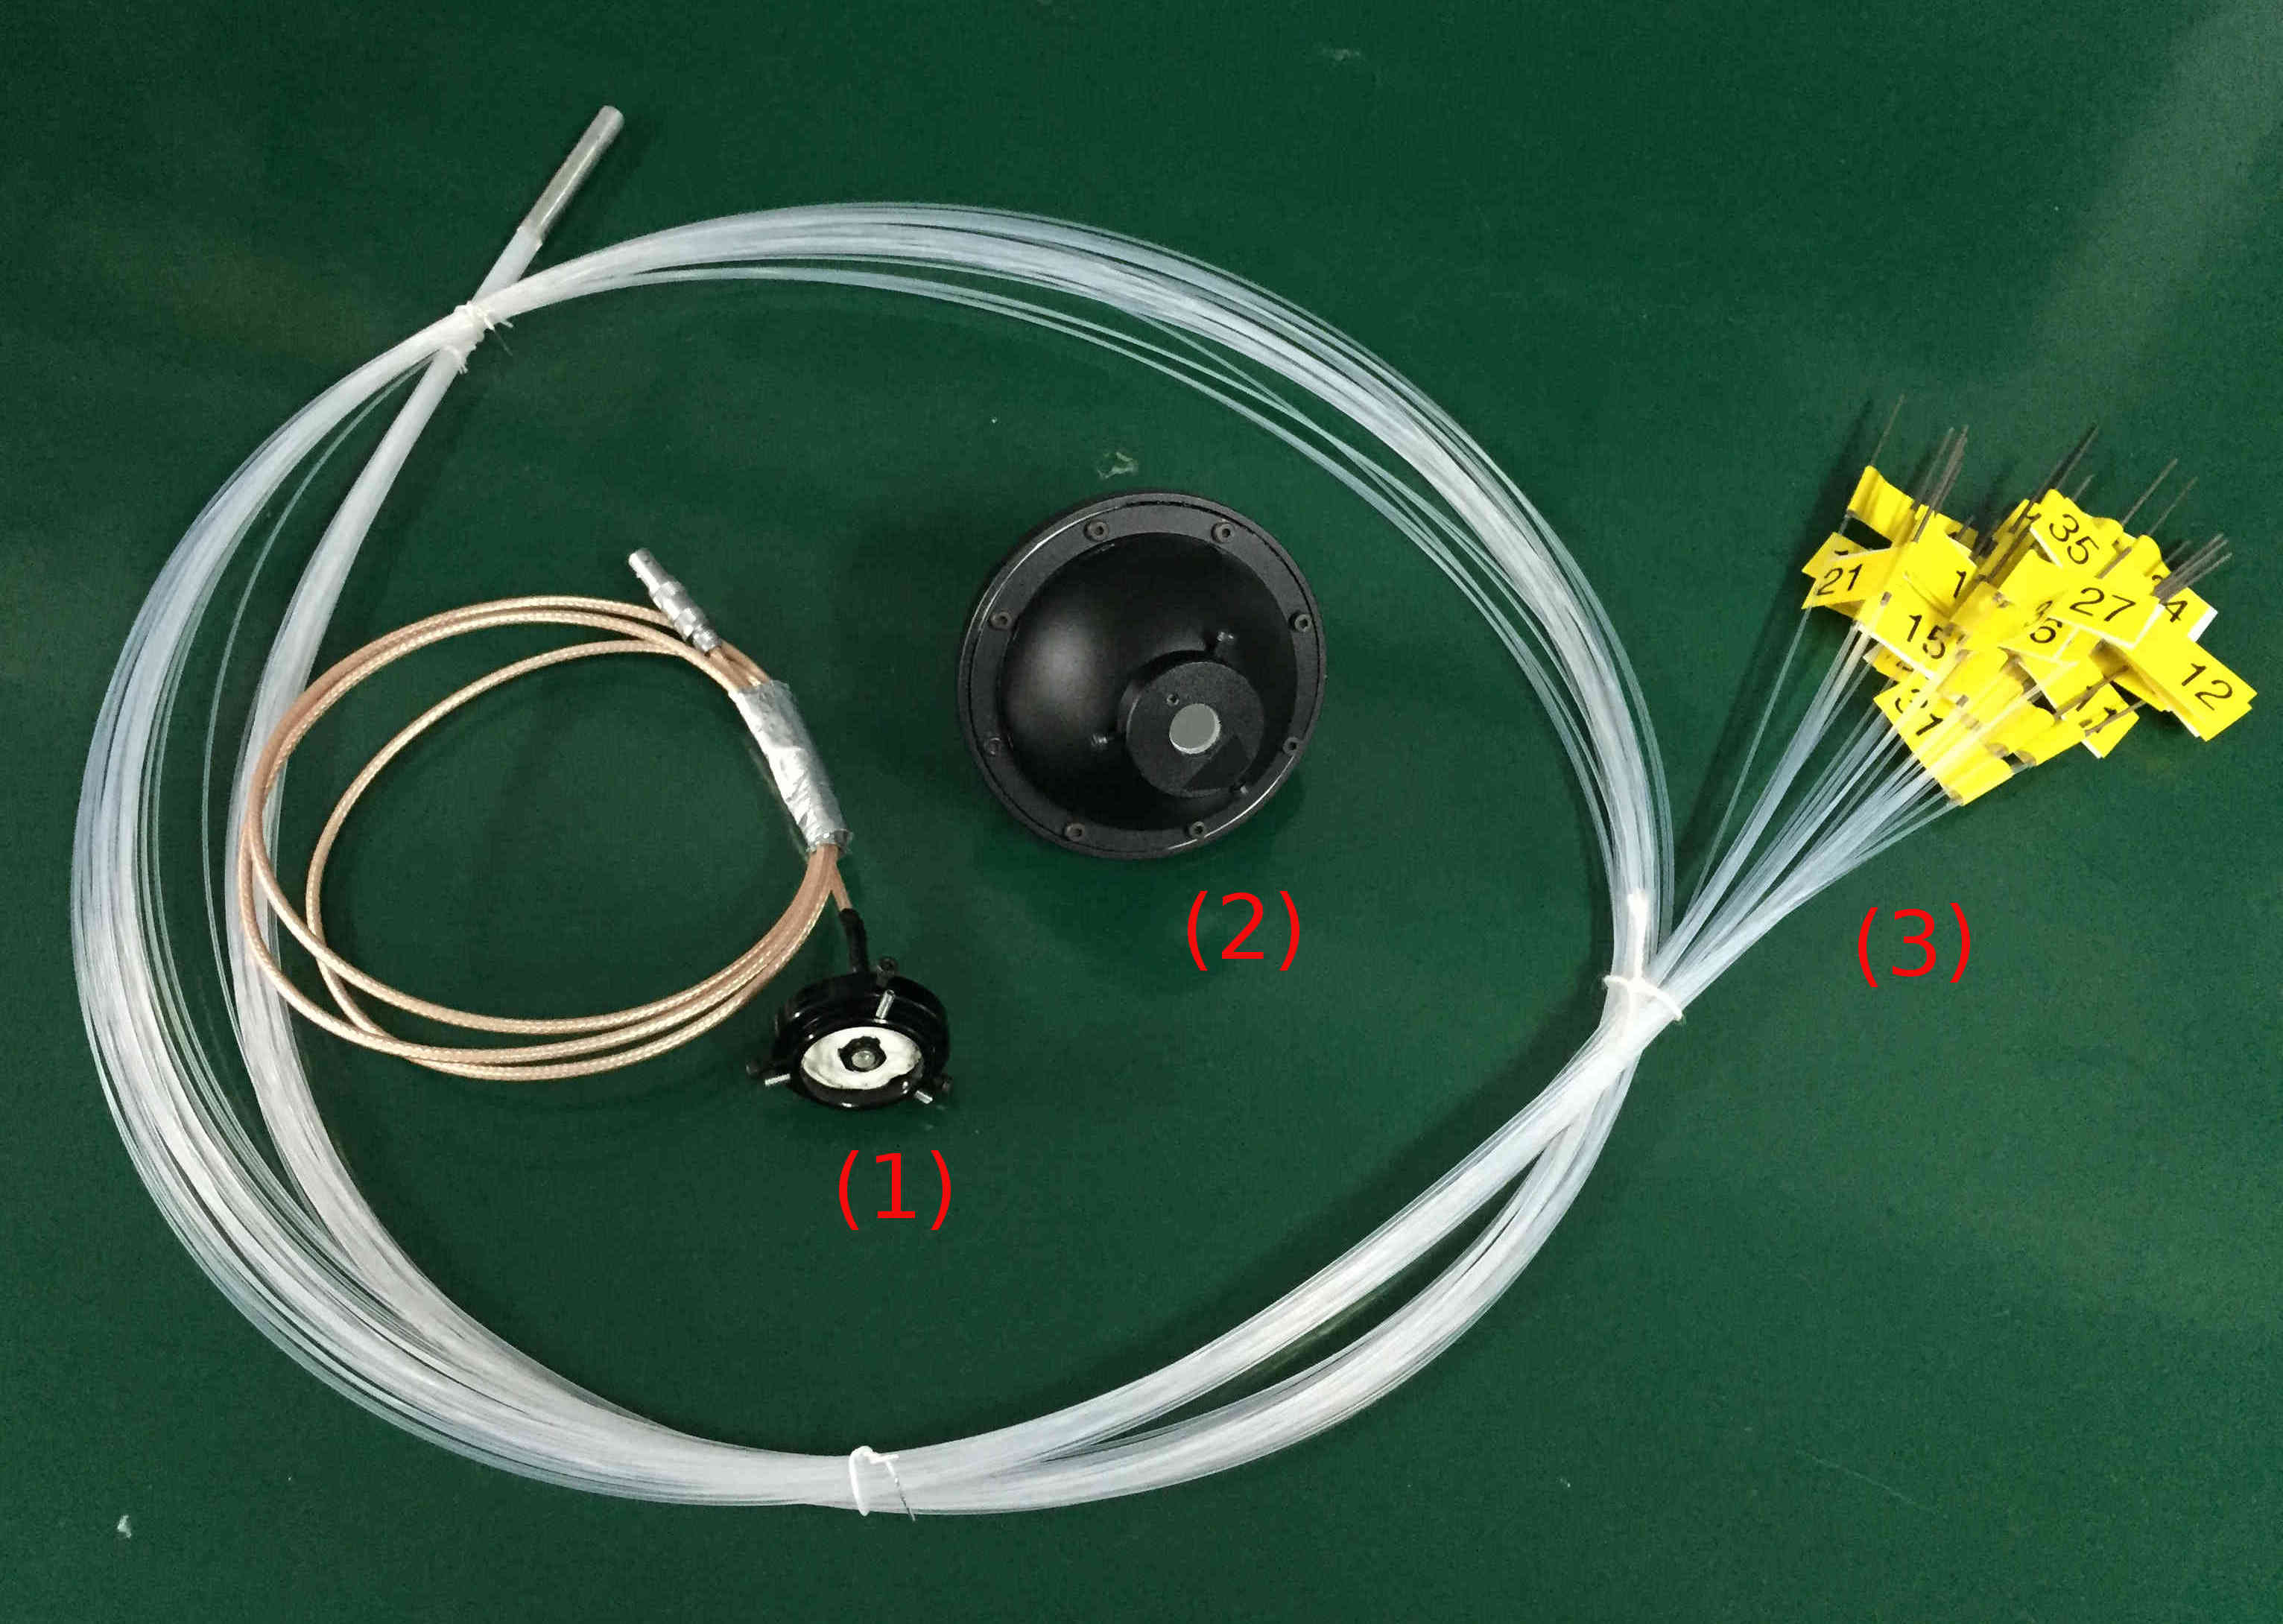
\includegraphics[width=0.49\textwidth]{chap/pmt_test/fig/lightsource_components.jpg}
	}
	\subfloat[][各组件耦合在一起]{
		\label{fig:pmt_test:lightsource_integration}
		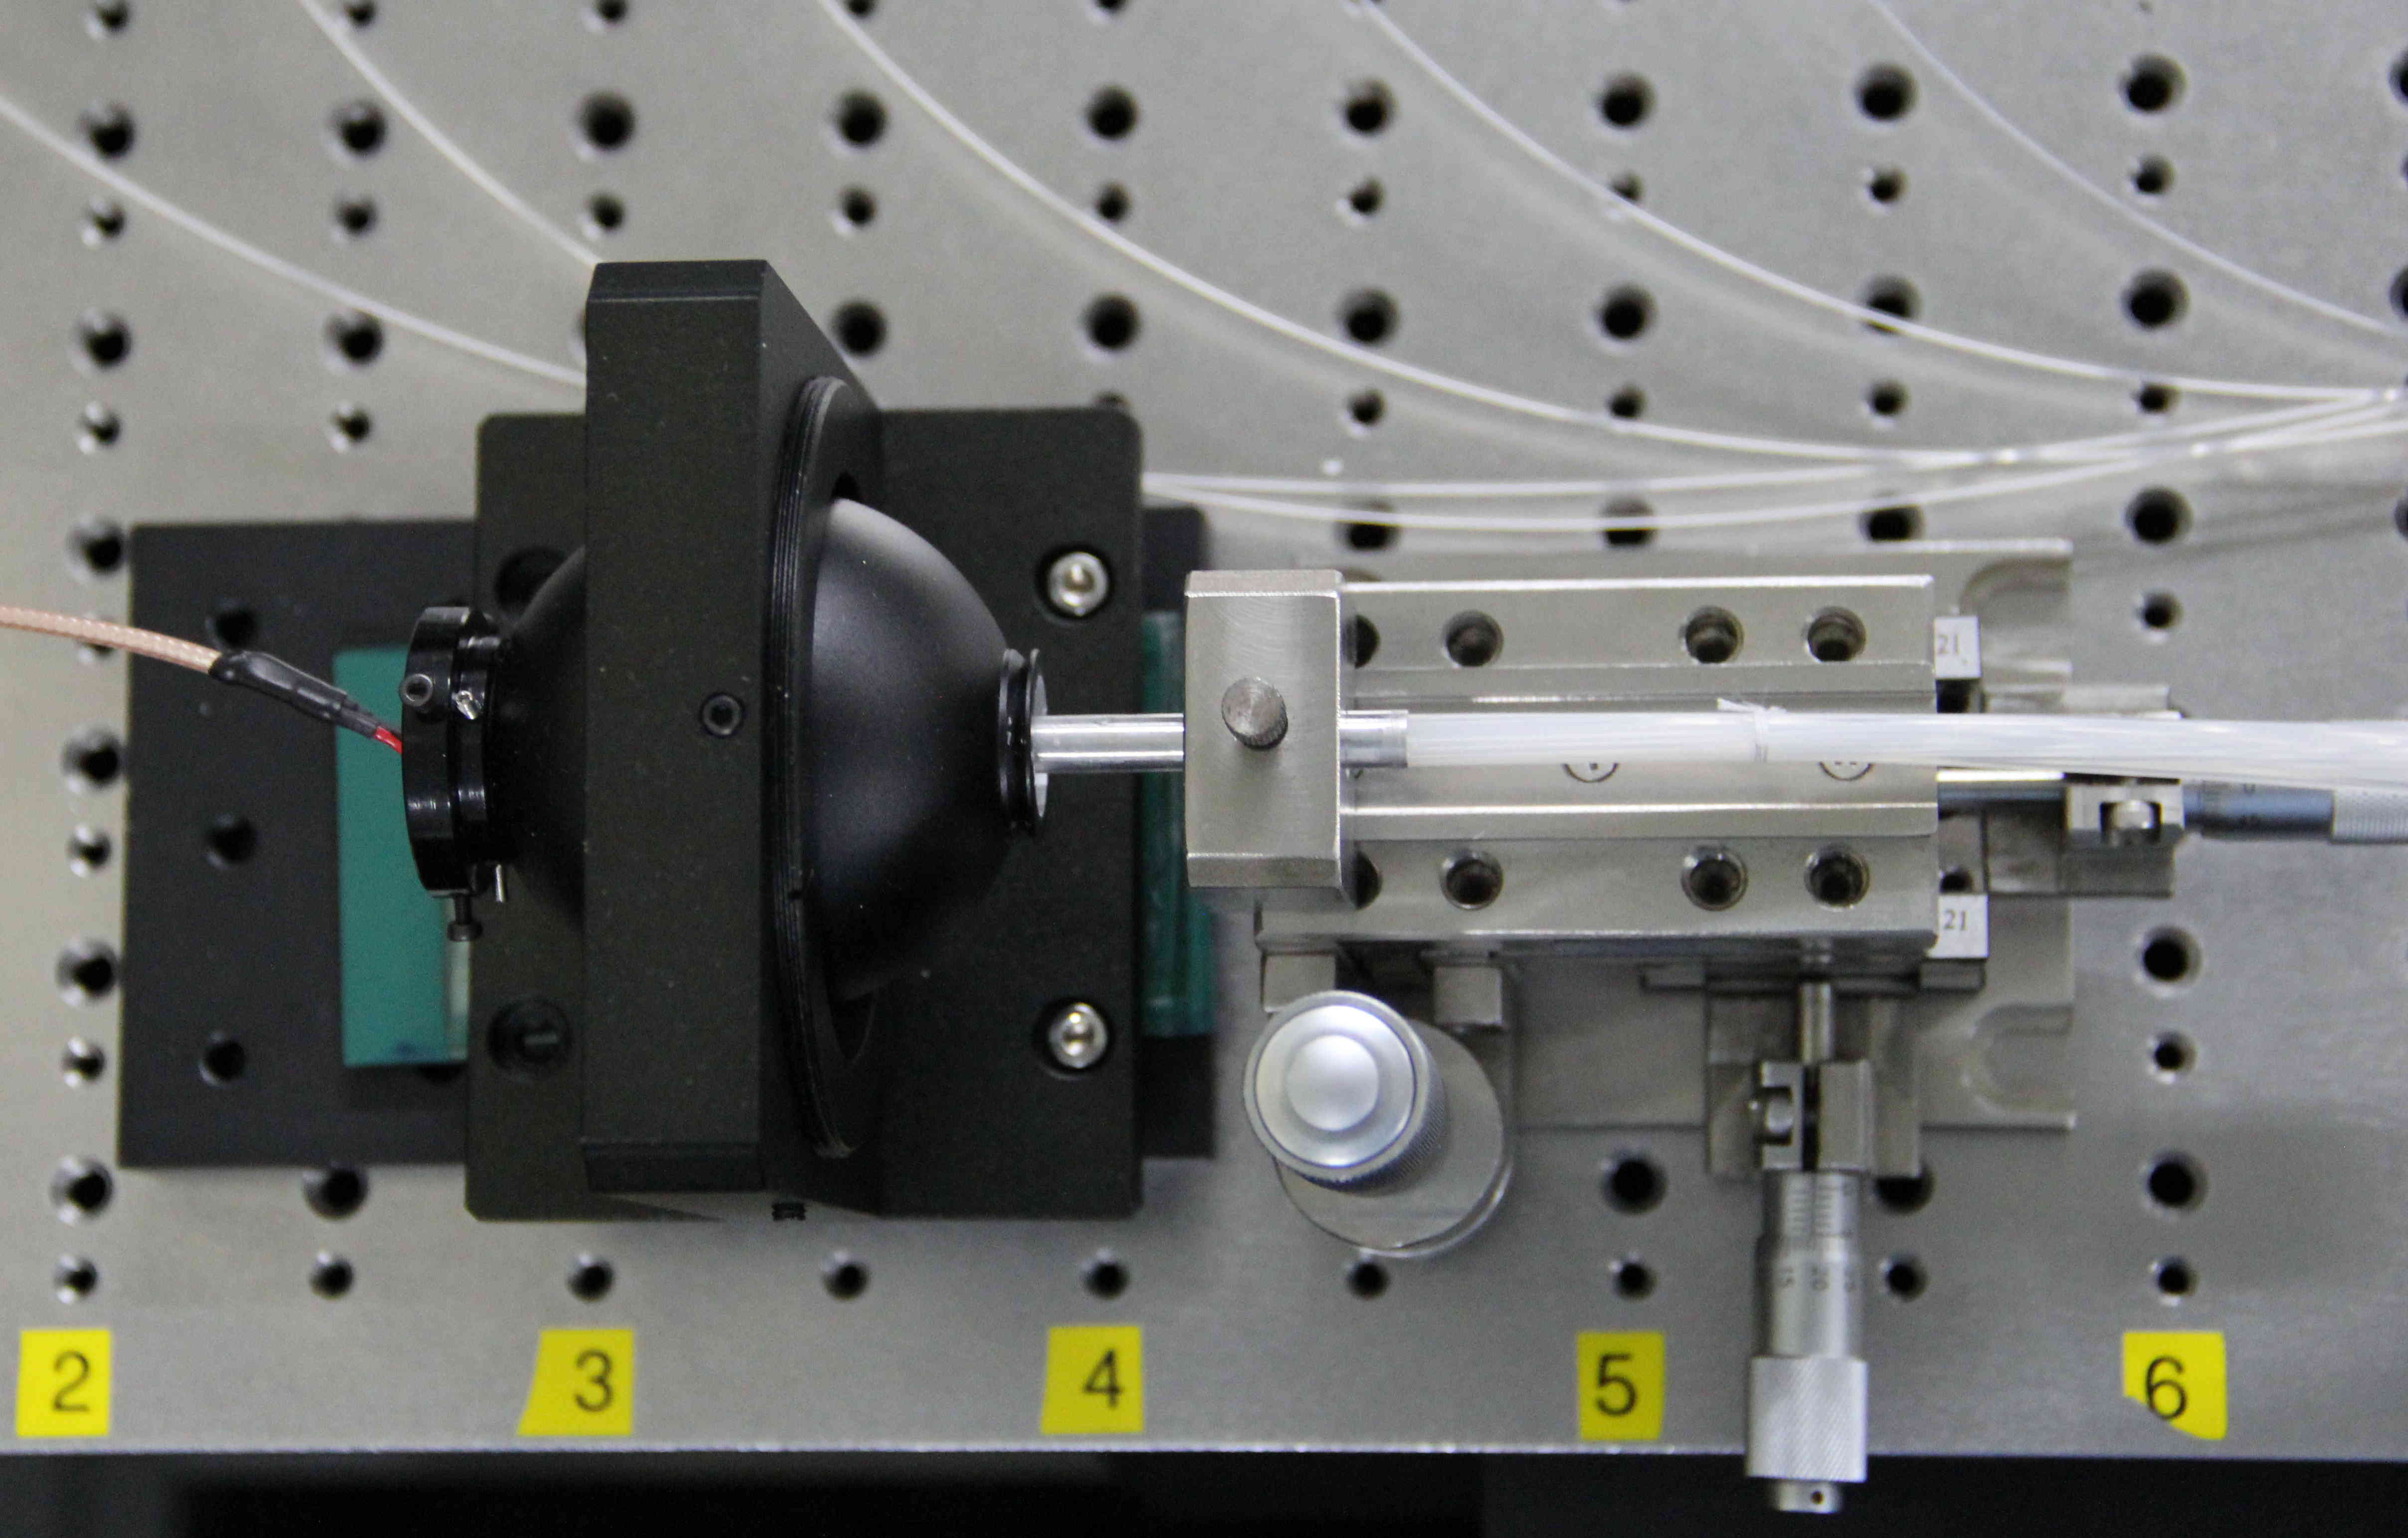
\includegraphics[width=0.49\textwidth]{chap/pmt_test/fig/lightsource_integration.jpg}
	}		
	\caption{PMT批量测试平台的光源与光分配系统}
	\label{fig:pmt_test:light_distribution}
\end{figure}
积分球是一个具有高反射性内表面的空心球体,它是一个理想的光积分器件,入射光在其内部经过多次反射后,能够在其出射端口均匀出射。
积分器在此处的应用主要出于两点考虑:1)我们希望各条光通路具有相近的光输出强度;2)方便积分球与集束光纤之间的耦合操作,减弱LED光源的非均匀性对各光路输出强度差异的影响。
我们使用的积分球\cite{integrating_sphere}使用的内壁涂层材料为$BaSO_4$,蓝光反射率达到\SI{98.5}{\percent},因此即便它的半径较小,仍然能够得到较好的均匀性。
在LED固定到积分球入射端口后,我们对积分球出射端面的光强度进行了“十”字扫描,结果显示其光均匀性可以达到$\pm\SI{0.5}{\percent}$,如图\ref{fig:pmt_test:integrationsphere_uniformity}所示。
\begin{figure}[htbp]
	\centering
	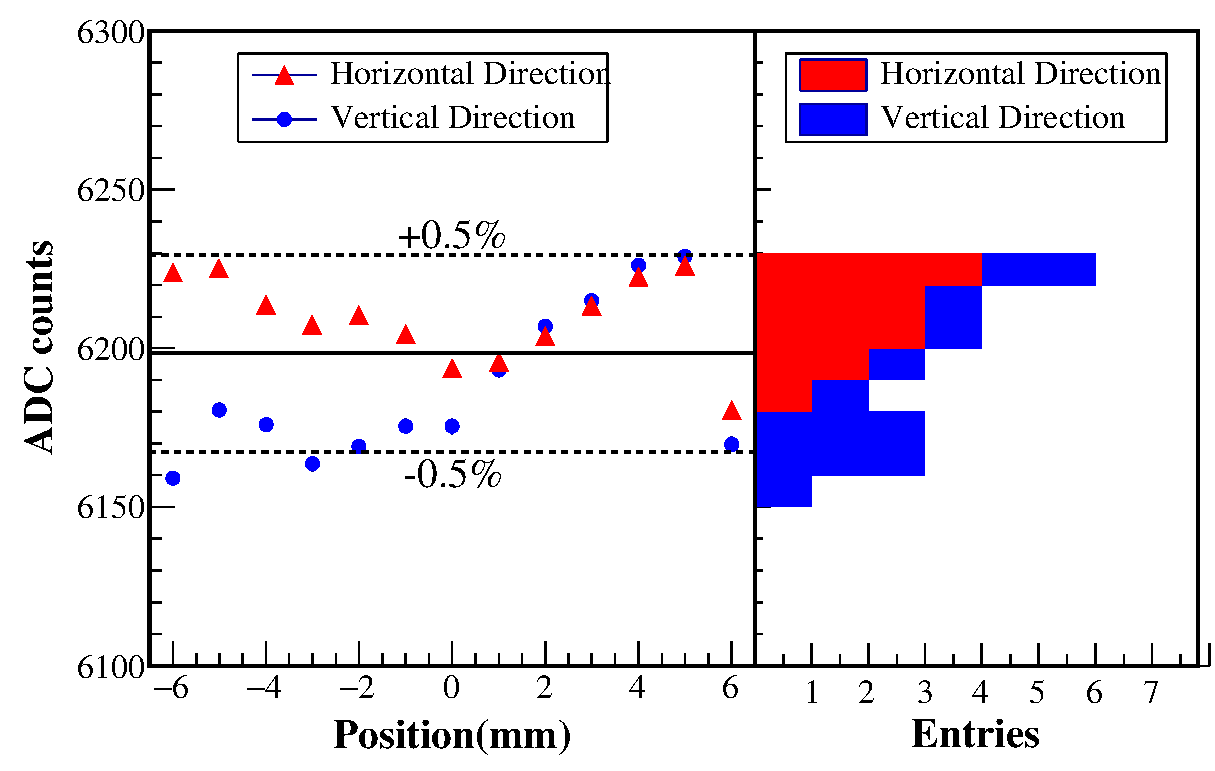
\includegraphics[width=0.65\textwidth]{chap/pmt_test/fig/integrationsphere_uniformity.eps}
	\caption{\SI{5}{cm}铝合金积分球输出端口的光均匀性}
	\label{fig:pmt_test:integrationsphere_uniformity}
\end{figure}

% 集束光纤
PMT批量测试系统使用的集束光纤由35根塑料包层的石英光纤\cite{optical_fibre}集结而成(25根用于待测光通道,2根用于监控光通道,剩余8根备份)。每根光纤的长度为\SI{1.5}{\meter},纤芯直径为\SI{400}{\micro\meter},包层厚度\SI{75}{\micro\meter},而数值孔径达到了$0.37$。
较大的芯径和数值孔径使得每条光通路都能从积分球中引出足够的光量,并传输到对应的PMT入射端面。
为了避免机械损伤,光纤的两个端头部位都加装了铝合金套筒进行保护,见图\ref{fig:pmt_test:lightsource_components}。
光源和光分配系统固定完成后,我们对35条光通路的输出光强差异进行了测试。
测试使用了两支R4443,一支管子用于监测LED的光强波动,其数值可以对测试结果进行光强校正;另一支管子用于正式测试,它固定不动而待测光纤使用高精度的光纤位移台调整位置,保证每次测试时待测光纤都能对准测试PMT光阴极的相同位置。
测试中,我们使用了两个不同幅度的LED驱动脉冲设置分别对所有光通路进行了扫描。
两种设置虽然有将近4倍的光强差,但它们得到的光强差异是在$\pm \SI{0.3}{\percent}$的范围内是完全一致的,结果如图\ref{fig:pmt_test:fiber_difference}所示。
\begin{figure}[htbp]
	\centering
	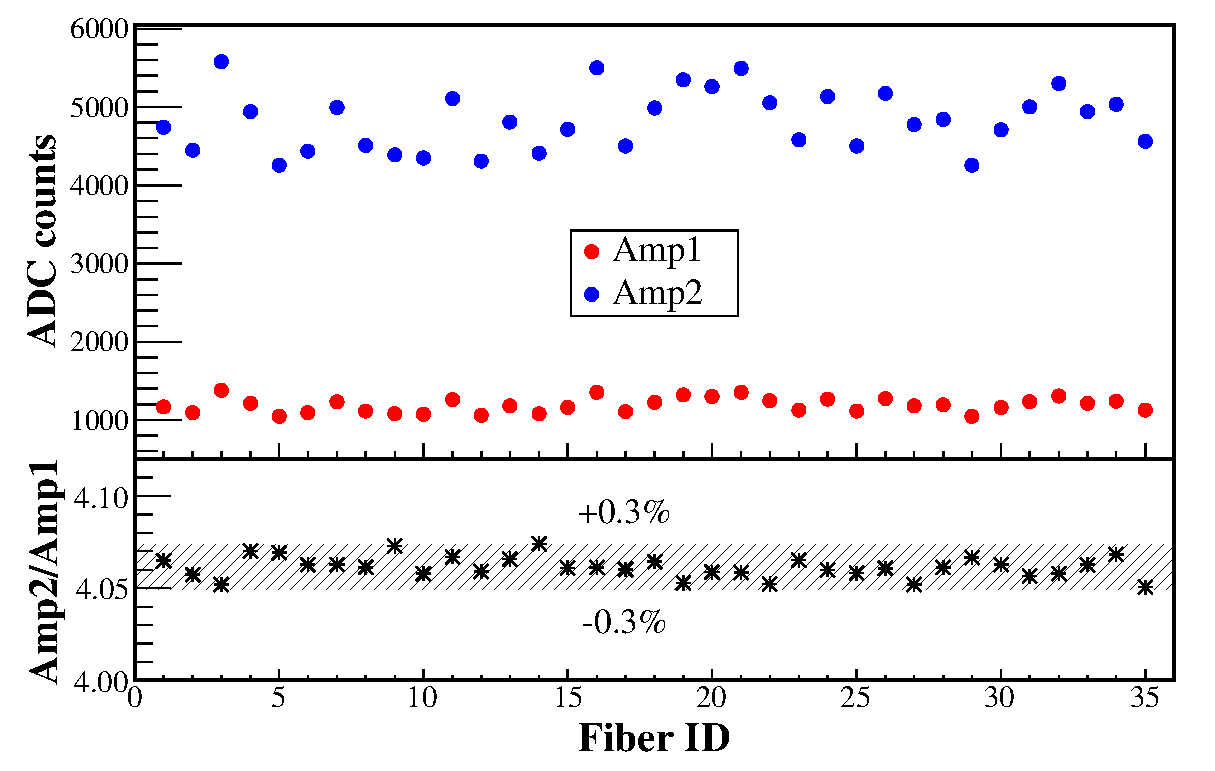
\includegraphics[width=0.7\textwidth]{chap/pmt_test/fig/fiber_difference.eps}
	\caption{集束光纤各通道的光传输差异性}
	\label{fig:pmt_test:fiber_difference}
\end{figure}
测试结果显示,所有光通路的输出光强度差异不大,但并不完全一致,其分布的标准差为\SI{10}{\percent}。
考虑到积分球的光输出分均匀性只有\SI{0.5}{\percent},可以认为各光通路的光输出强度差异主要是光纤自身的传输效率差异导致的。
由于传输效率是光纤的固有特征,其在相当长的一段时间内是比较稳定的,可以认为是个常数。
假设本次测试中,编号为$fiberid$的光纤输出光强度为$L_{fiberid}$,同时在所有光通道中选择一个作为参考通道,其输出光强度为$L_{ref}$。
则编号为$fiberid$的光通道的光输出强度差异系数$\tau_{fiberid}$可以定义为:
\begin{equation}
	\tau_{fiberid} = \frac{L_{fiberid}}{L_{ref}}
	\label{eq:pmt_test:lightoutput_difference}
\end{equation}
根据上面的叙述,$\tau_{fiberid}$可以被认为是一个常数,它主要用于对测试数据进行光强校正,使得不同光通道的测试结果可以直接进行比较(详见第\ref{sec:pmt_test:characterization}节)。

\subsection{模块化设计的测控软件}
\label{sec:pmt_test:software}
% 最好这里做一个归纳性的介绍,具体细节设计放到附录中
PMT批量测试平台的测控软件是系统的重要组成部分,它直接关系到平台的易用性。
由于该测试平台被设计为是一个通用的测试系统,我们需要考虑很多潜在的测试内容,并且底层硬件需要经常更换或更新(见\ref{sec:pmt_test:testbench_functions}的描述)。
因此,PMT批量测试平台的测控软件框架采用模块化的设计思路,并对底层硬件进行了封装和虚拟化,从而方便软件进行维护以及扩展。
测控软件框架基于C++语言编写,并在Windows环境下运行,其内部组件可以被分为以下三个层级:
\begin{enumerate}
	\item 设备的抽象层。分别用一个C++的抽象类代表\ref{sec:pmt_test:testbench_functions}节中介绍的四个功能模块,并将各种模块常用的操作抽象出来作为借口函数。任何一个新加入的设备都可以从这四个抽象类中继承出来,并对提供自己接口函数实现。软件框架里的其余部分可以通过这四个抽象类来完成自己的功能,并不涉及其具体实现,从而将底层硬件与顶层功能隔离开来。
	\item 测试算法与辅助功能库。这一层提供了一些基于上述的设备抽象层实现的一些较为通用的测试用例算法,以及一些管理类和辅助功能类。
	\item 用户交互层。这一层主要处理和用户的交互,其具体实现与上两层无关,可以基于命令行,也可以基于图形界面。
\end{enumerate}
测控软件框架的具体设计细节可以参看附录\ref{appendix:pmttest_software},此处略去。
对于PSD的光电倍增管测试来说,我们基于NI-VISA\cite{ni_visa}函数库实现了对PSD地面检测获取系统的控制,以代替通用的CAMAC数据获取模块。
针对PSD的测试需求,实现了Dy8增益测试、Dy5和Dy8的相对增益测试以及光阴极扫描测试这三个测试算法。
最后,我们基于PDCurses\cite{pdcurses}开发了一个命令行交互的测控程序,集成了设备控制,状态监控以及日志记录等功能。

\section{PSD对光电倍增管的测试需求}
\label{sec:pmt_test:test_requirement}
由于PSD没有参加DAMPE的触发系统,不需要对粒子的入射时间进行测量,因此R4443的时间性能参数没有实际的参考价值,无须对其进行专门的测试。
另一方面,PSD通过测量沉积能量的大小来实现其所有功能(见第\ref{sec:description:psd_principle}节),而光电倍增管的增益是直接影响探测器能量响应的重要参数。
因此,我们对R4443的测试主要集中在与增益相关的性能参数,包括Dy8的增益以及Dy8和Dy5之间的相对增益(简称Dy58比值)两个方面。

% 能量响应均匀性的要求
PSD要求各探测单元模块的对MIP粒子的中心能量响应均匀性好于\SI{25}{\percent}(见\ref{sec:description:psd_requirements}),这意味着PSD上安装的所有R4443需要有相近的Dy8增益值。
PSD使用双打拿极引出信号来实现其动态范围的覆盖,各探测单元模块的动态范围不能太小以致不能探测$Z=20$的Ca离子,动态范围也不能太大以致降低了能量测量的分辨率,浪费读出电子学的有效测量范围。
因此,PSD对动态范围覆盖区间大小进行了严格的限制,这意味着Dy8的增益确定下来后,Dy58比值也就基本确定下来了,即PSD上安装的所有R4443也需要有相近的Dy58比值。
一般来讲,我们可以通过改变分压器工作电压的大小来调节光电倍增管的增益值,使其满足探测器设计要求。
光电倍增管各打拿极或阳极的增益$G$与分压器工作电压$V$之间满足幂函数关系,即
\begin{equation}
	G = A V^\alpha
	\label{eq:pmt_test:gain_powerfunction}
\end{equation}
其中,$A$和$\alpha$都是常数。
由于Dy5的增益也是工作电压的幂函数,可以进一步推得Dy58比值$G_{58}$也是分压器工作电压的幂函数:
\begin{align}
	G_{58} &= \frac{G_{dy8}}{G_{dy5}} = \frac{A_{dy8}}{A_{dy5}} V^{\alpha_{dy8}-\alpha_{dy5}}      \\
		   &= A' V^{\alpha'}
	\label{eq:pmt_test:dy58_powerlaw}
\end{align}
其中,$A'$和$\alpha'$也是常数。
在本文中,将上述两个关系分别定义为R4443的Dy8增益特性曲线以及R4443的Dy58比值增益特性曲线。
如果我们能够通过测试确定这两条特性曲线,就能根据增益需求反推出每支R4443的工作电压,为PSD的建造和运行提供参考。
这也是我们对PSD的R4443光电倍增管进行性能测试的主要目标。

% 高压分组使得需要对大量管子进行测试
PSD中每6/7支PMT组成一个高压分组,共享一路高压通道;而且,DAMPE高压单机的输出电压不能连续调节,只有7个工作档位,档位间隔为\SI{30}{V}(详见\ref{sec:description:psd_hv})。
这就要求同一高压分组内的所有R4443,在相同的工作电压下具有相近的增益值。
另外,DAMPE的设计寿命是3年,在这么长时间的持续辐照条件下,塑闪单元条和光电倍增管的寿命都会受到影响;在运行后期,塑闪单元条的发光效率会降低,而光电倍增管的增益系数也有可能减小,此时需要调高高压档位,以维持PSD的整体探测性能。
这就进一步要求每个高压分组内的R4443还要有相近的Dy8增益特性曲线和Dy58比值增益特性曲线,使得它们在工作电压换挡后也能够保持相近的增益值,从而保证各单元模块的能量响应差异和动态范围覆盖区间不产生大的波动。
如前所述,光倍增管的个体差异较大。
为了满足上述两个要求,我们需要对大量候选PMT进行性能测试,然后根据得到增益特性曲线对这些PMT进行筛选和分组,才能选出PSD正式需要的164支PMT。

\section{R4443的性能测试及结果}
\label{sec:pmt_test:characterization}
\subsection{测试综述}
\label{sec:pmt_test:characterization_summary}
% 高压分组导致从570支 选194 最后用164
% 统计信息 20一个run 共28个run 一个月测试完成
% 测试流程: 预热
我们使用PMT批量测试平台,共对570只R4443进行了完整的性能测试,图\ref{fig:pmt_test:testbench_withpmt}显示了所有待测PMT固定到测试平台后的样子。
\begin{figure}[htbp]
	\centering
	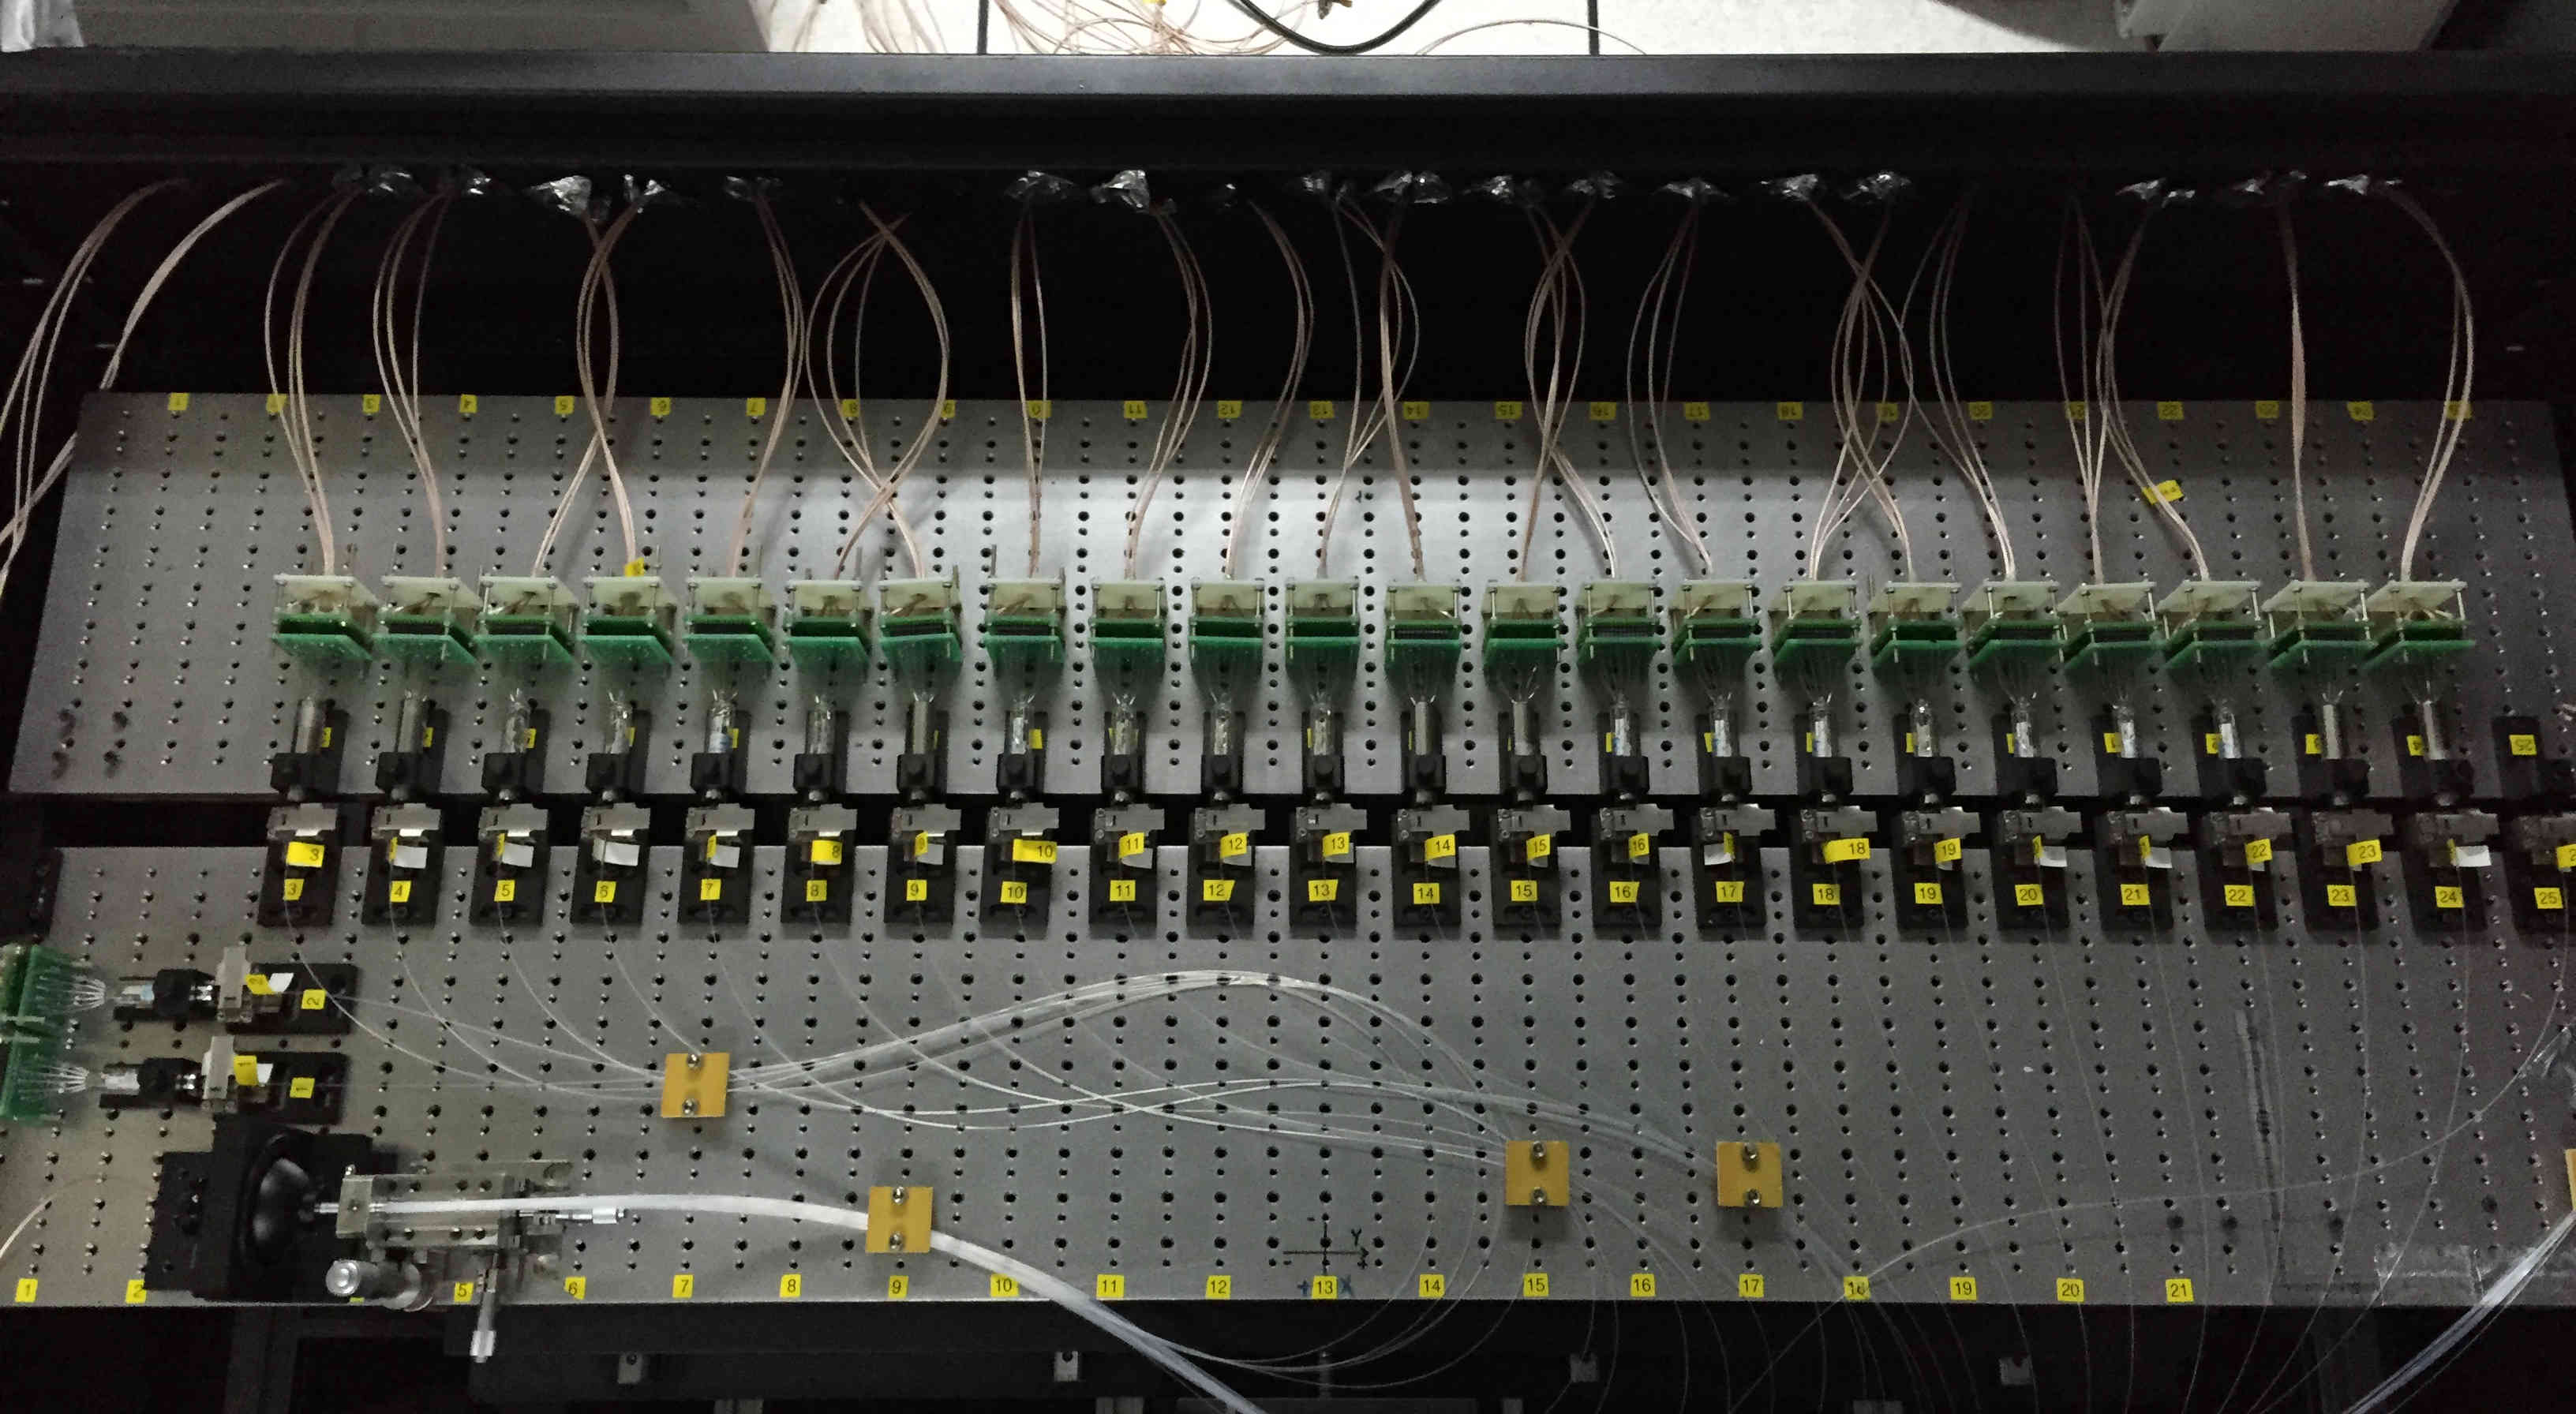
\includegraphics[width=0.9\textwidth]{chap/pmt_test/fig/testbench_withpmts.jpg}
	\caption{PMT安装到PMT批量测试平台后等待测试}
	\label{fig:pmt_test:testbench_withpmt}
\end{figure}
测试分成28个Run进行,每个Run对将近20支管子同时进行测试,在一个月内完成全部测试工作。
一次Run需要花费5.5个小时,其中包括一个小时的PMT安装/拆卸,两个小时的PMT加电预热以及两个半小时的正式测试。
测试内容主要包括Dy8相对增益得测量和Dy58比值的测量,我们还对部分管子进行了光阴极扫描,以考察R4443光阴极不均匀性对测试结果的影响。

% 分压器:可复用
% 获取系统组成,数据分析,数据库存储
为了得到最真实的测试结果,测试中使用的分压器电路以及前端电子学处理电路与PSD实际使用的完全一致。
另外,我们还专门设计了可重复使用的Base电路板,以方便PMT的安装与拆卸,如图\ref{fig:pmt_test:baseboard}所示。
它包含基座板和分压器板两个部分:基座板提供信号转接的功能,它上面没有元器件,并直接焊接到R4443管脚上,每个管子一个;分压器板包含完整的分压器电路,它被固定在测试平台上,每个测试通道一个。
基座板和分压器板之间通过可直接插拔的排针连接在一起,这样就方便了PMT的安装与拆卸。
由于不是所有待测的管子都会被安装到PSD上,这也减少了分压器板的需求量。
\begin{figure}[htbp]
	\centering
	\subfloat[][R4443裸管焊接到基座板上]{
		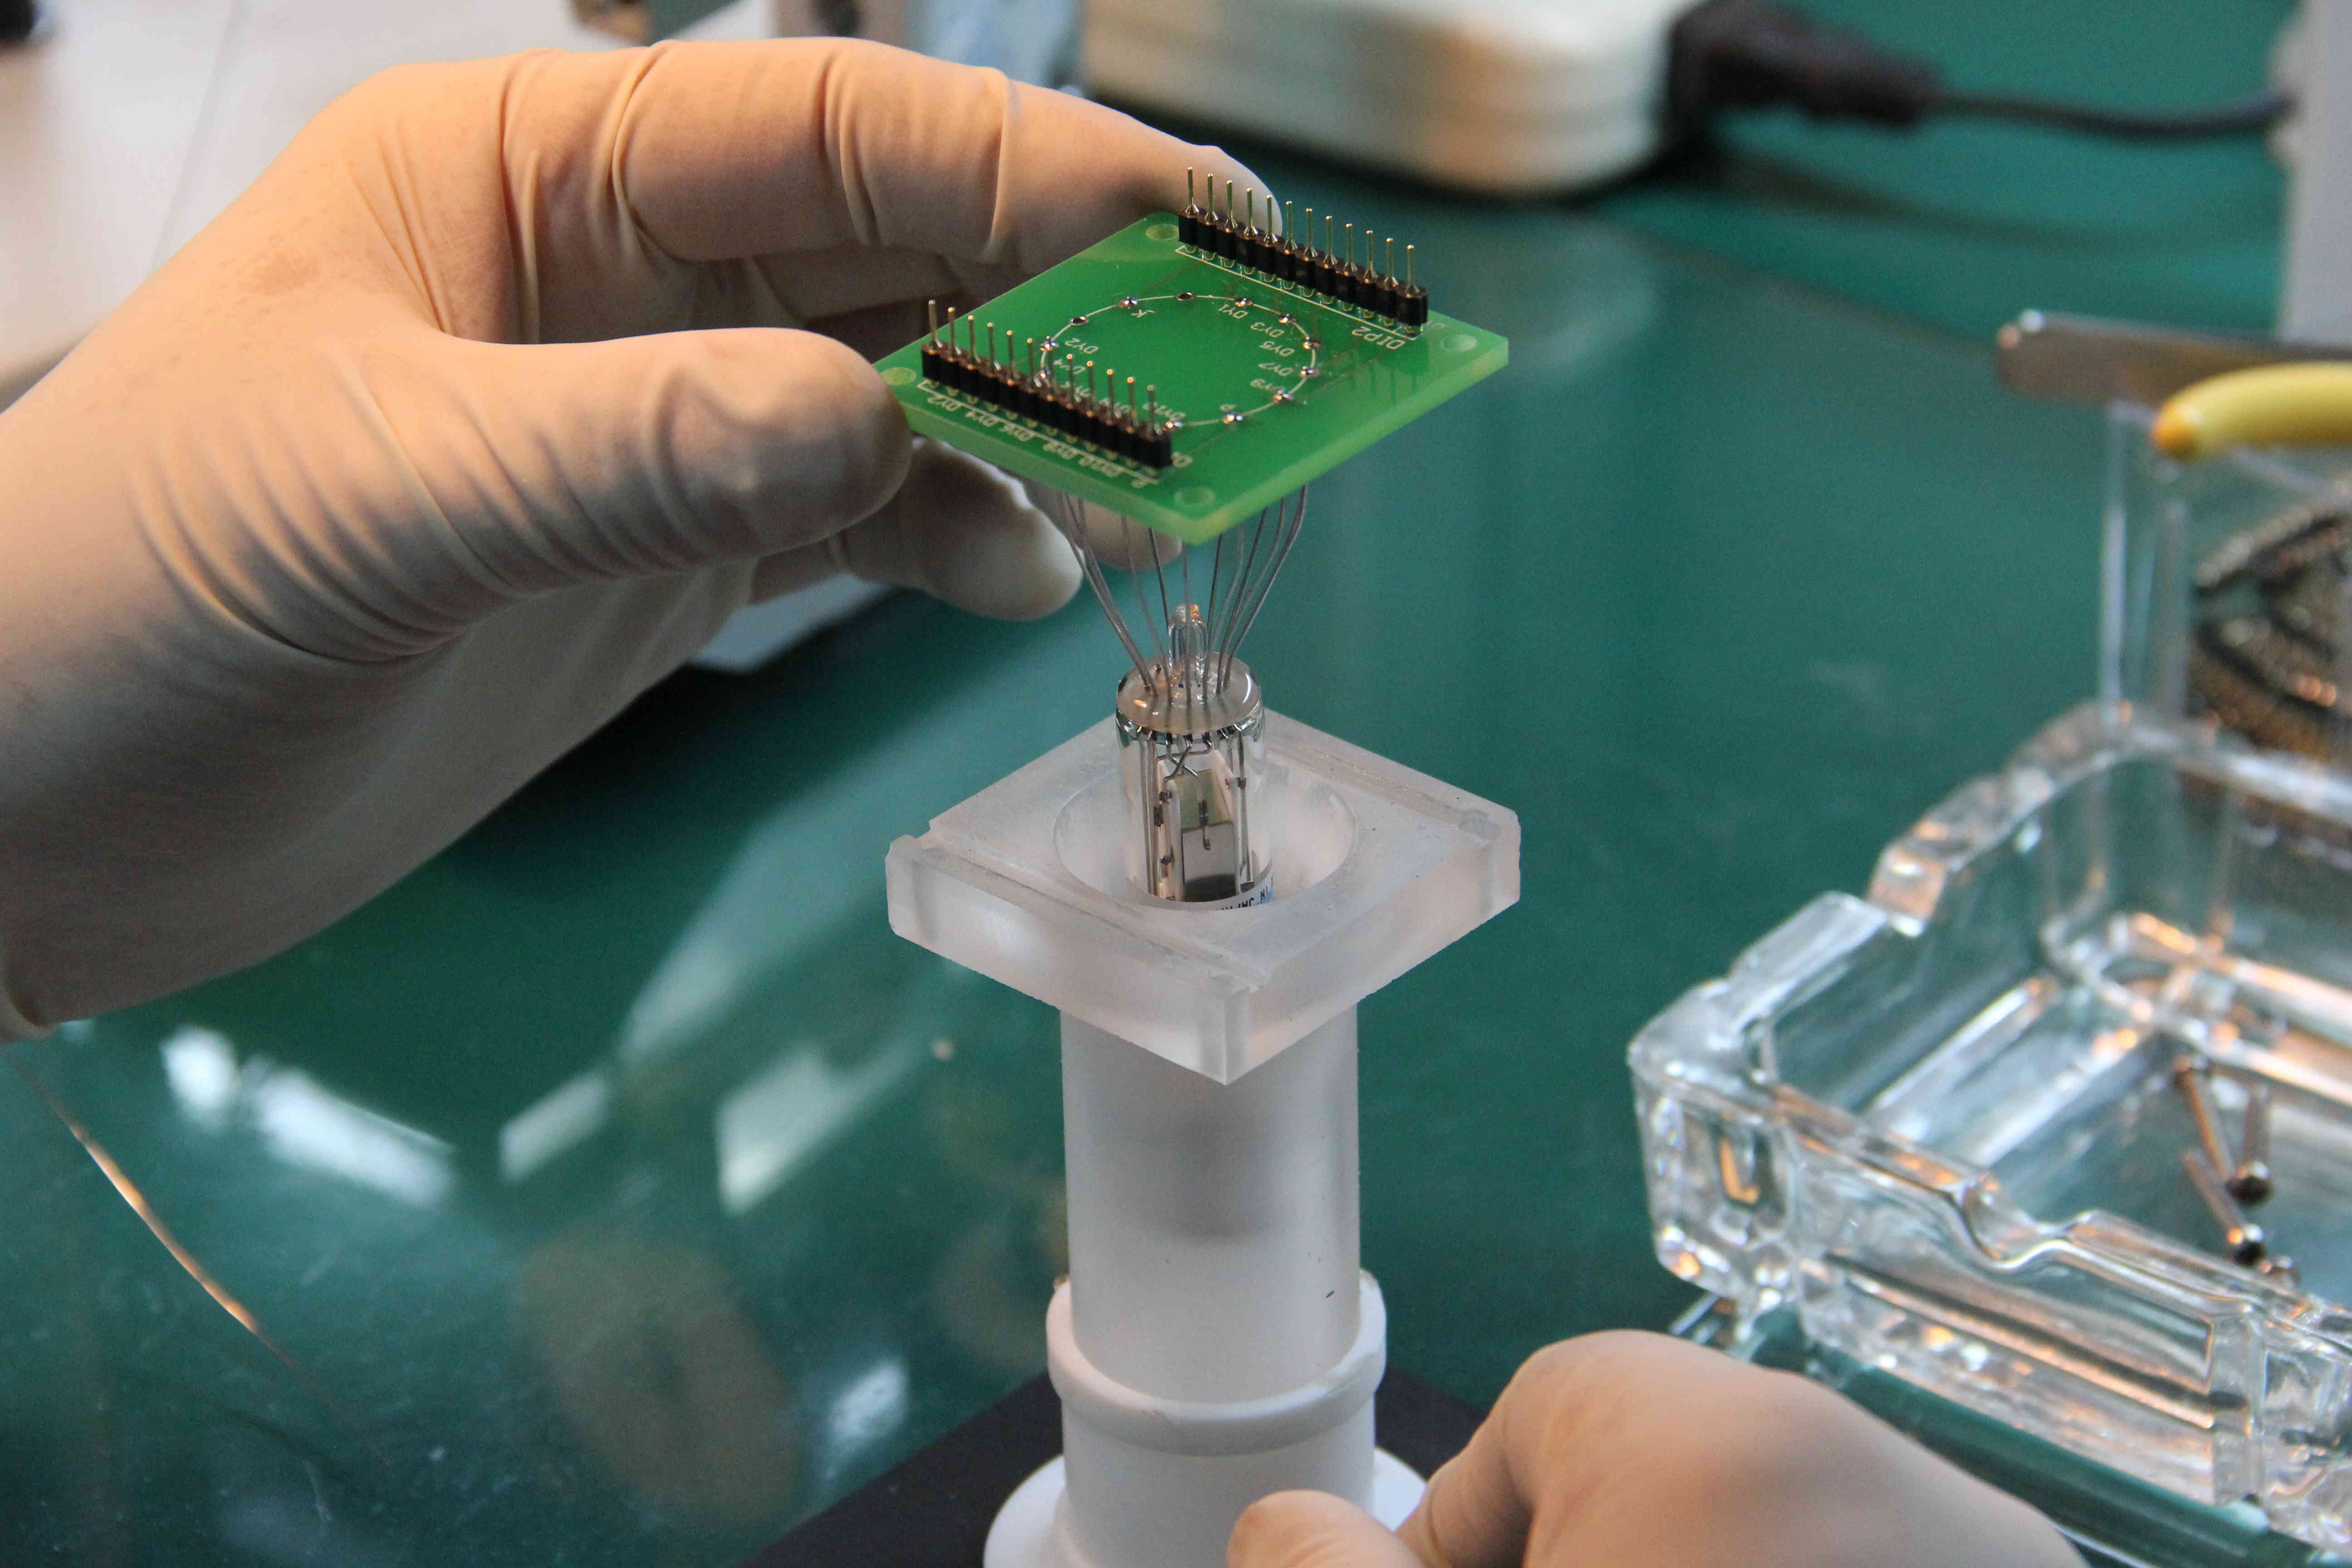
\includegraphics[width=0.48\textwidth]{chap/pmt_test/fig/base_board_a.jpg}
		\label{fig:pmt_test:baseboard_a}
	}
	\subfloat[][基座板与分压器板通过排针连接成一个整体]{
		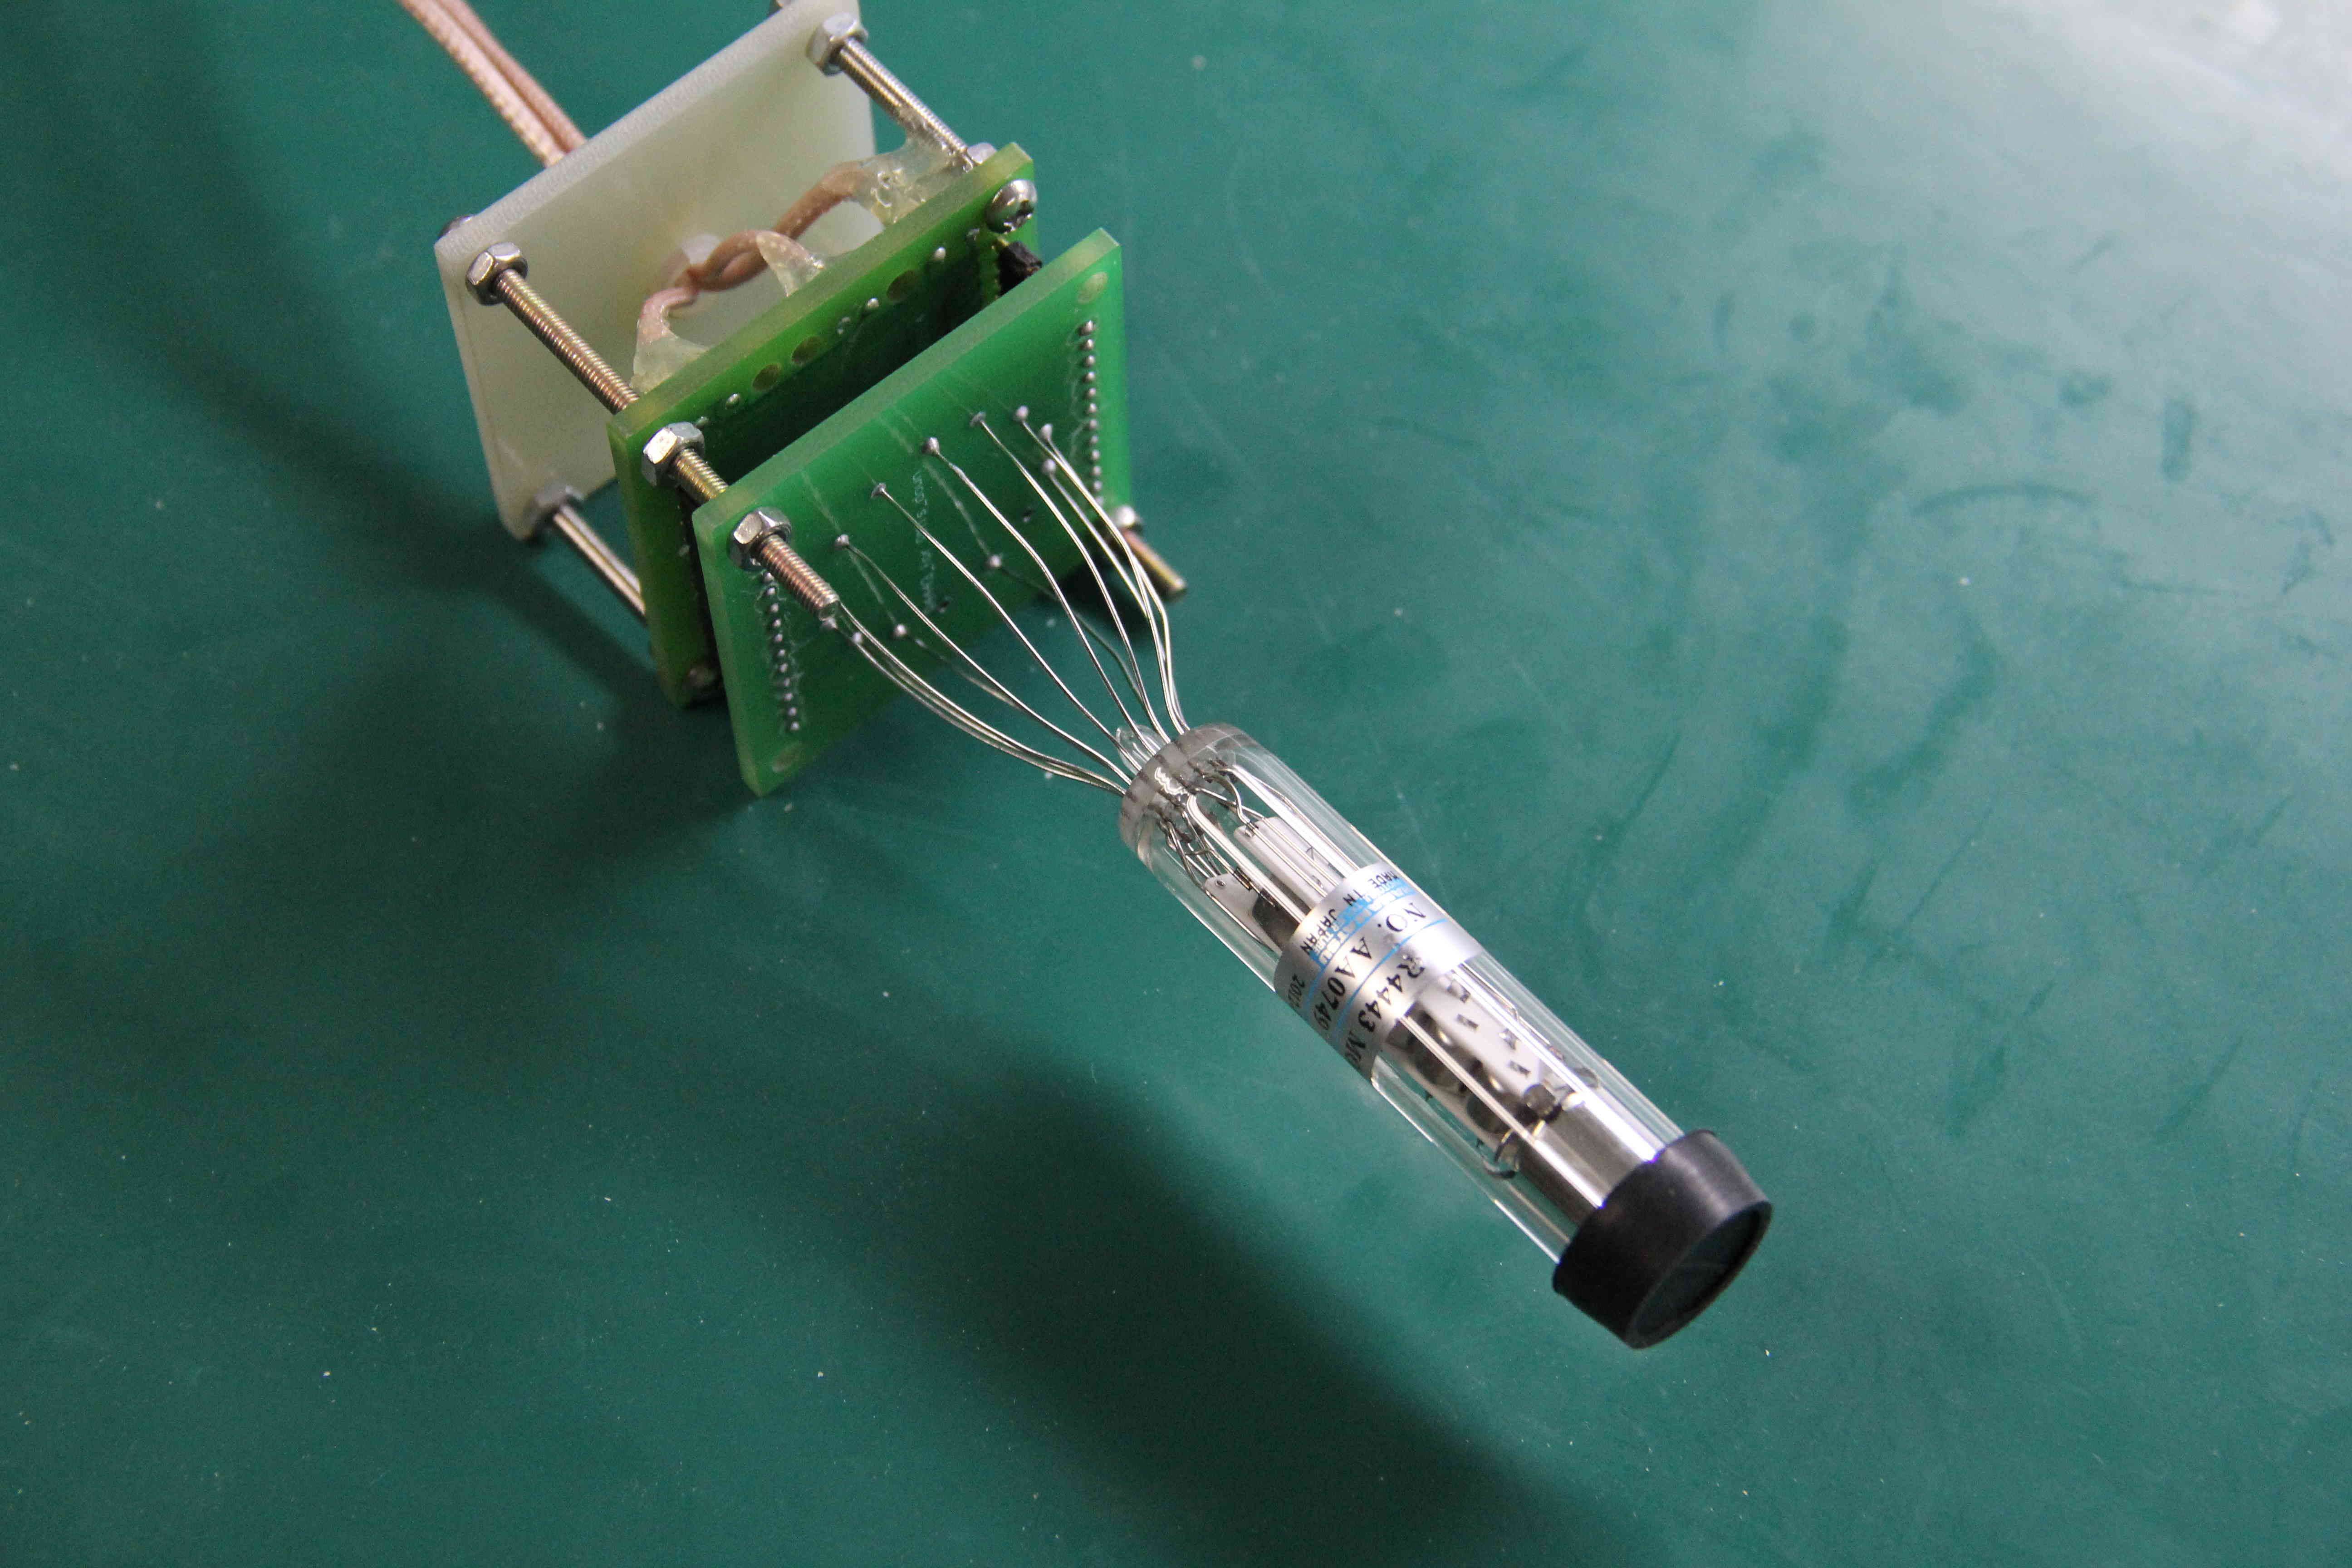
\includegraphics[width=0.48\textwidth]{chap/pmt_test/fig/base_board_b.jpg}
		\label{fig:pmt_test:baseboard_b}
	}
	\caption{用于R4443性能测试的Base电路板}
	\label{fig:pmt_test:baseboard}
\end{figure}

\subsection{Dy8相对增益的测量}
\label{sec:pmt_test:relative_gain}
% 测试方法的介绍:
测量光电倍增管增益最常用的方法是:用极弱的脉冲光源照射PMT得到其单光电子谱,然后拟合其峰位得到绝对增益大小。
然而,这种方法并不适合测量PSD中R4443管子的Dy8增益,这是因为:1)R4443第8打拿极的增益较小,使用PSD的FEE板虽然可以在较高的工作电压下得到单光电子响应谱,但在工作电压较低时其单光电子谱并不明显,因此不能确定Dy8增益随工作电压的变化关系;2)通过单光电子峰位得到的增益只是PMT电子倍增器部分的绝对增益,并不包含光阴极和聚焦电极的贡献,而PMT的实际增益是这两部分的累加,因此这种测试方法并不全面。

由于单光电子方法的上述限制,我们采用了另一种方法对R4443第8打拿极的增益进行测量,即使用相同强度的光脉冲照射PMT,然后根据Dy8输出信号的电荷量大小来确定其增益。
这种方法得到的结果并不能得到光电倍增管的绝对增益,只能通过比较不同管子间的信号大小得到它们之间的相对增益,因此本文将其称为相对增益测量方法。
在表述相对增益方法得到的测试结果时,一般选取一支光电倍增管作为参考,取其它管子相对于这支管子的信号比值作为相对增益测量值,以消除测试结果对入射光强度的关联,即:
\begin{equation}
	G_{relative} = \frac{L\cdot G_{abs}}{L\cdot G_{ref}} = \frac{G_{abs}}{G_{ref}}
	\label{eq:pmt_test:relative_gain}
\end{equation}
其中,$L$表示入射光强度,$G_{abs}$和$G_{ref}$分别是待测PMT和参考PMT的绝对增益。
之后,可以对这支参考光电倍增管的具体性能进行更加细致的测试,如绝对增益,这样其它管子的相关性能也就能根据相对增益测量值反推得到。
在PSD的应用中,我们将参考PMT耦合到塑闪单元条上,通过寻找最佳的MIP响应来确定它的额定工作电压,最终反推出其它管子的额定工作电压(详见第\ref{ch:construction}章)。

% 校正说明
相对增益测量方法的关键是产生相同强度的光脉冲。
对于我们使用的PMT批量测试平台来说,主要有两点需要考虑:
\begin{itemize}
	\item LED光源的稳定性。 虽然我们可以设置AFG3252每次都使用相同的驱动脉冲设置,但LED是半导体器件,它对环境温度较为敏感,因此其光输出强度会出现波动。PMT批量测试平台中有两支监控PMT用于LED光输出强度的监测,因此我们可以利用它们的测试数据对不同次Run的LED输出光强进行校正归一。我们将第$runid$次Run相对于第一个Run得到的校正系数定义为$k_{runid}$。
	\item 不同光通道的输出光强度差异。 根据\ref{sec:pmt_test:testbench_hardware}节的测试结果,我们知道不同光通道的输出光强并不相同,其差异系数为$\tau_{fiberid}$。由于$\tau_{fiberid}$是个常数,我们可以用它将不同测试通道的输出光强归一化。
\end{itemize}
因此,在数据处理中,我们需要对原始数据进行上述两种因素的校正,才能得到准确的测量结果。
假设PMT批量测试平台测得的信号原始谱峰位为$A_{raw}$,则校正后的结果$A_{corr}$可以表示为:
\begin{equation}
	A_{corr} = \frac{A_{raw}}{\tau_{fiberid} k_{runid}}
	\label{eq:pmt_test:gain_correction}
\end{equation}

% 流程、配置介绍
使用上述方法,我们以\SI{50}{V}为间隔,从\SI{700}{V}到\SI{1000}{V}选取了七个电压点对相对增益进行了扫描,以得到每个管子的Dy8增益特性曲线。
为了保证不应幅度超出R4443的线性范围而导致测试数据无效,我们使用了5个不同强度的光脉冲进行相对增益的测量。
我们发现在线性范围内,不同入射光强度得到的相对增益是一致的,但是随着电压或光强度的增加,Dy8输出信号越来越趋近饱和,此时不同光强得到的相对增益会有差别,如图\ref{fig:pmt_test:gain_twointensity_correlation}所示。
\begin{figure}[htbp]
	\centering
	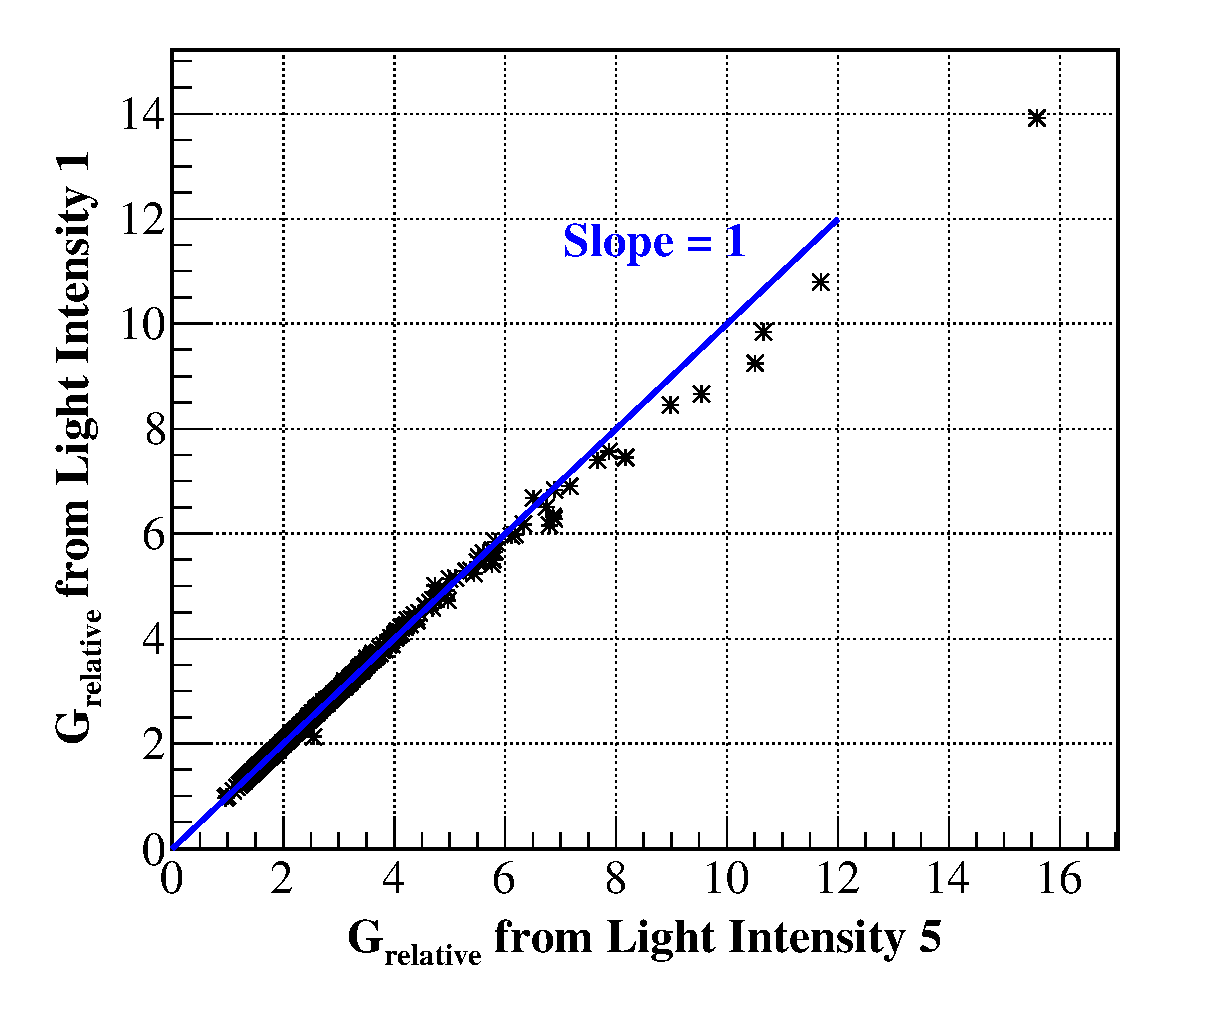
\includegraphics[width=0.65\textwidth]{chap/pmt_test/fig/gain_twointensity_correlation.eps}
	\caption{在\SI{850}{V}工作电压下,最大光强度(Light Intensity 1)和最小光强度(Light Intensity 5)得到的相对增益关联图。可以看到增益很大的管子,最小光强得到的增益要略大于最大光强得到的增益。}
	\label{fig:pmt_test:gain_twointensity_correlation}
\end{figure}
数据处理时,我们舍去接近饱和区域的幅度测量点,只取在所有电压范围内数据都有效的数据点进行分析,最终得到了所有待测管子的增益特性曲线。
图\ref{fig:pmt_test:gain_vs_voltage}给出了两支PMT的测试结果作为示例,其中实线是使用公式\ref{eq:pmt_test:gain_powerfunction}拟合的结果,它们都能很好地符合幂函数变化规律。
根据测得的增益特性曲线,我们可以计算出R4443在任意工作电压下PMT的相对增益大小,图\ref{fig:pmt_test:gain_distribution_850}给出了\SI{850}{V}时570只管子的Dy8增益分布。
\begin{figure}[htbp]
	\centering
	\subfloat[][本次测试得到的Dy8增益特性曲线]{
		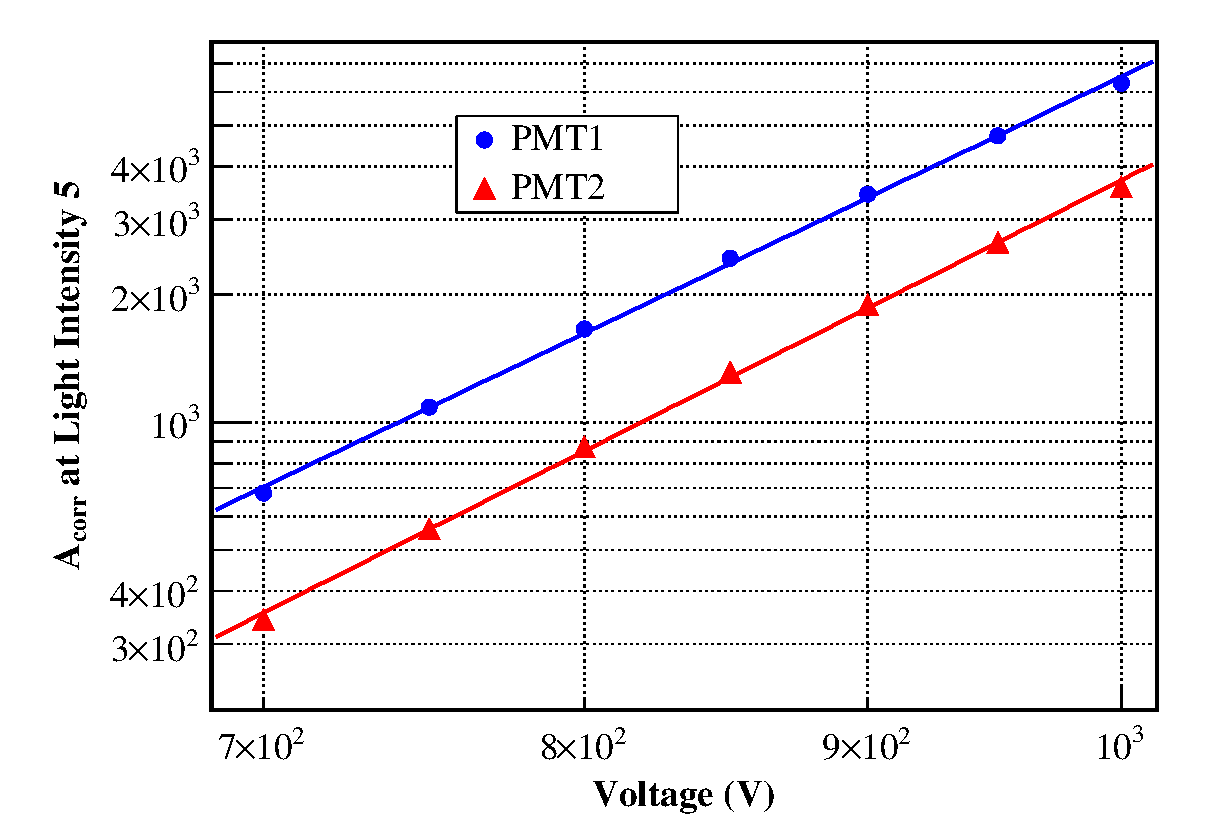
\includegraphics[width=0.5\textwidth]{chap/pmt_test/fig/gain_vs_voltage.eps}
		\label{fig:pmt_test:gain_vs_voltage}
	}
	\subfloat[][\SI{850}{V}工作电压下,所有管子的相对增益分布,选择增益最小的管子作为参考PMT]{
		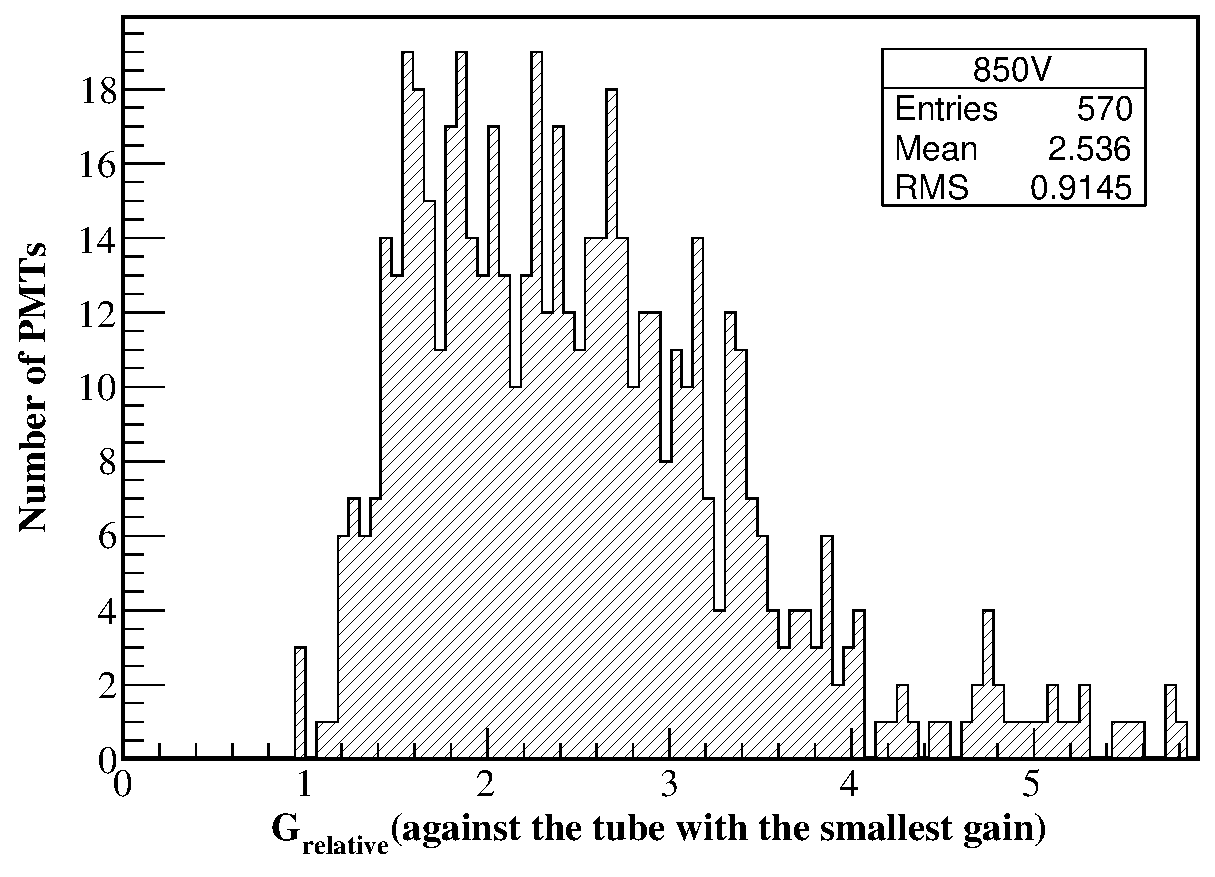
\includegraphics[width=0.5\textwidth]{chap/pmt_test/fig/gain_distribution_850.eps}
		\label{fig:pmt_test:gain_distribution_850}
	}
	\caption{Dy8相对增益的测量结果}
	\label{fig:pmt_test:gain_results}
\end{figure}

% 结果介绍
我们进一步将本次测试得到的结果与Hamamatsu提供的蓝光灵敏度测量结果进行了比较,如图\ref{fig:pmt_test:gain_vs_bluesensitivity}所示。
\begin{figure}[htbp]
	\centering
	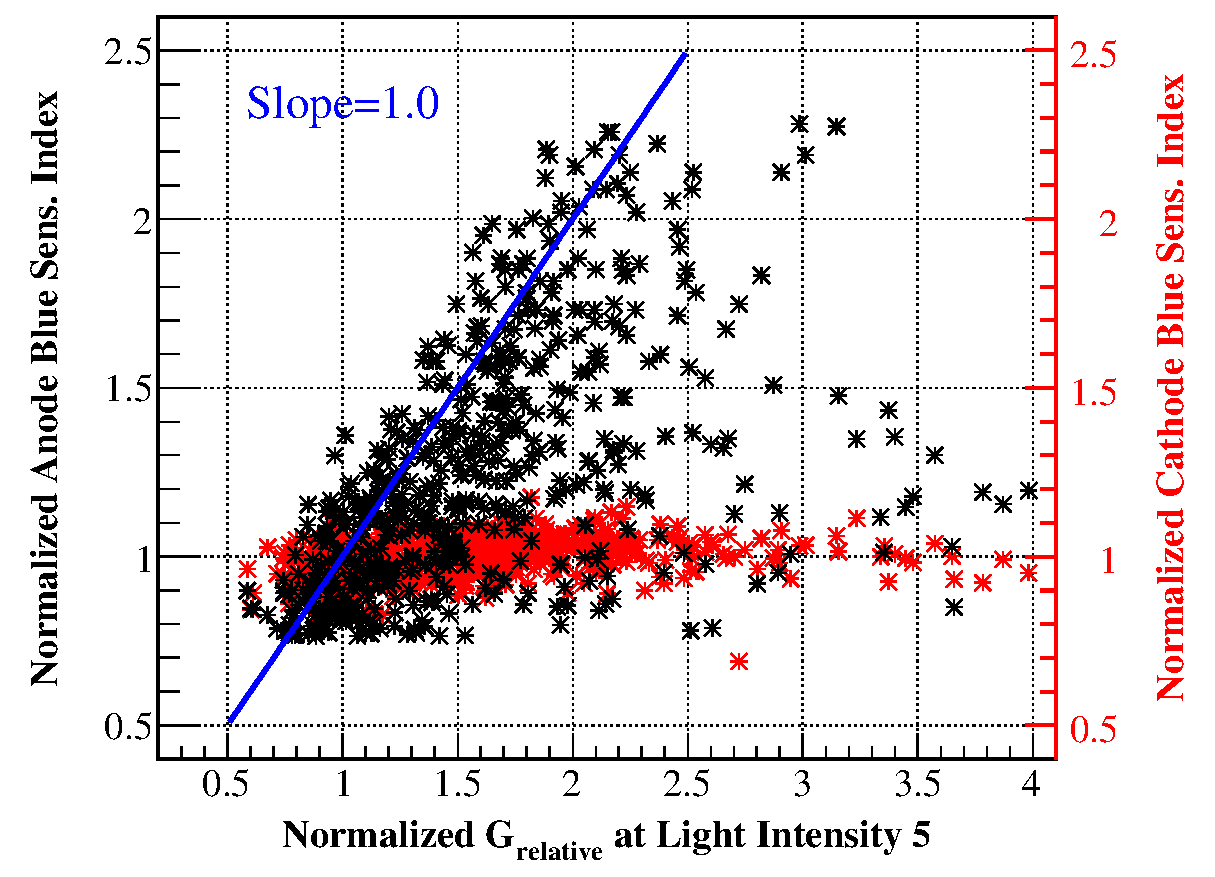
\includegraphics[width=0.65\textwidth]{chap/pmt_test/fig/gain_vs_bluesensitivity.eps}
	\caption{本次测试得到的Dy8增益与厂家提供的蓝光灵敏度的关联图。其中横轴是根据测得的增益特性曲线计算出的相对增益,纵轴左边黑色坐标是阳极蓝光灵敏度,右边红色坐标是阴极蓝光灵敏度。}
	\label{fig:pmt_test:gain_vs_bluesensitivity}
\end{figure}
为使比较更加准确,我们根据出厂测试使用的分压器和工作电压推出了PSD分压器上应该加载的等效电压,并根据测得的增益特性曲线计算出此时的相对增益。
并且为了便于比较,这三组数据都对同一支参考管子进行了归一。
可以看到,我们的结果与阴极蓝光灵敏度的关联性不强,而与阳极蓝光灵敏度具有近似为1的线性关联。
由于阳极蓝光灵敏度和我们的测量结果都包含了光阴极、聚焦极和电子倍增器的贡献,而阴极蓝光灵敏度只包含光阴极和聚焦极的贡献,该结果也就从侧面证明了相对增益测量方法的有效性和准确性。

\subsection{Dy8和Dy5之间相对增益的测量}
\label{sec:pmt_test:dy58}
Dy8与Dy5之间的相对增益测量比较简单:选取一系列不同强度(从弱到强,知道Dy8通道饱和)的光脉冲依次照射待测PMT,每个强度下分别记录Dy8和Dy5的信号大小,最终可以得到Dy8和Dy5的线性关联谱直到Dy8通道饱和,谱图的斜率就是Dy58比值,如图\ref{fig:pmt_test:dy58_example_single}。
\begin{figure}[htbp]
	\centering
	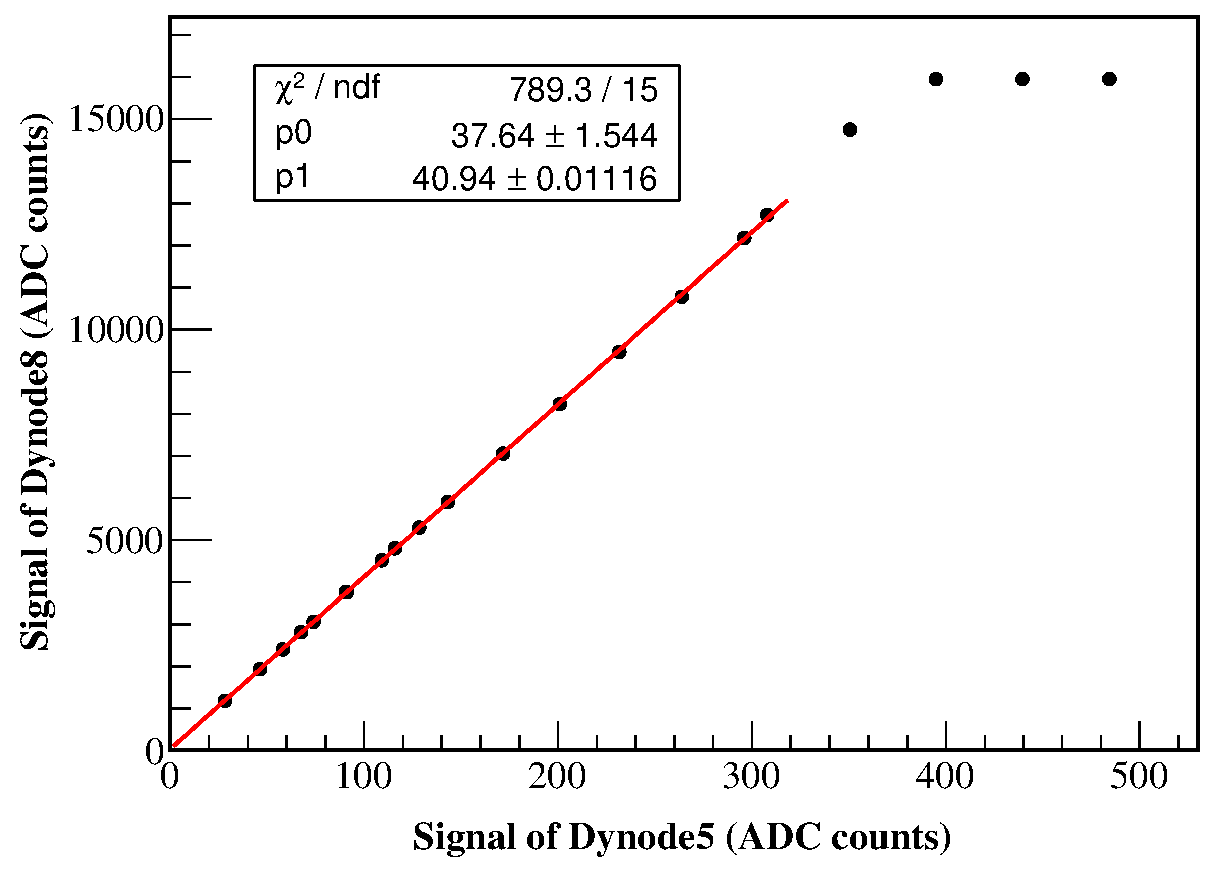
\includegraphics[width=0.65\textwidth]{chap/pmt_test/fig/dy58_example_single.eps}
	\caption{LED测试得到的Dy58曲线}
	\label{fig:pmt_test:dy58_example_single}
\end{figure}

同样地,我们以\SI{50}{V}为间隔,从\SI{700}{V}到\SI{1000}{V}选取了七个电压点对Dy58比值进行了扫描。
将七个电压点的数据整合在一起,使用公式\ref{eq:pmt_test:dy58_powerlaw}进行拟合,就得到了Dy58比值的增益特性曲线。
图\ref{fig:pmt_test:dy58_example}给出了一个示例,其中黑色圆点、蓝色三角以及红色星点分别是\SI{1000}{V}、\SI{850}{V}以及\SI{700}{V}下测得的Dy58曲线,小图是对七个电压下Dy58比值的幂函数拟合,可以看到数据点与拟合结果符合得非常好。
\begin{figure}[htbp]
	\centering
	\subfloat[][Dy58比值测试的一个示例]{
		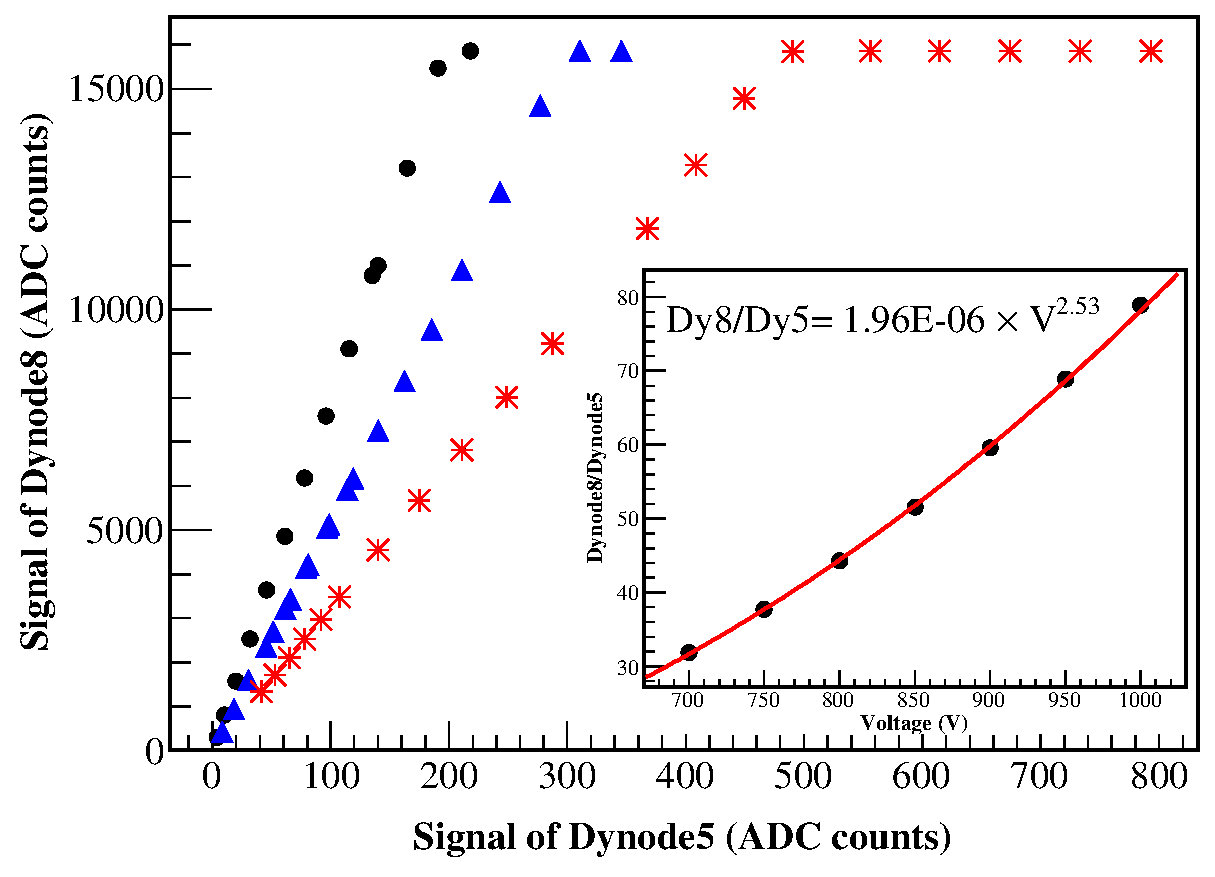
\includegraphics[width=0.49\textwidth]{chap/pmt_test/fig/dy58_example.eps}
		\label{fig:pmt_test:dy58_example}
	}
	\subfloat[][\SI{850}{V}工作电压下所有测试管子的Dy58比值分布]{
		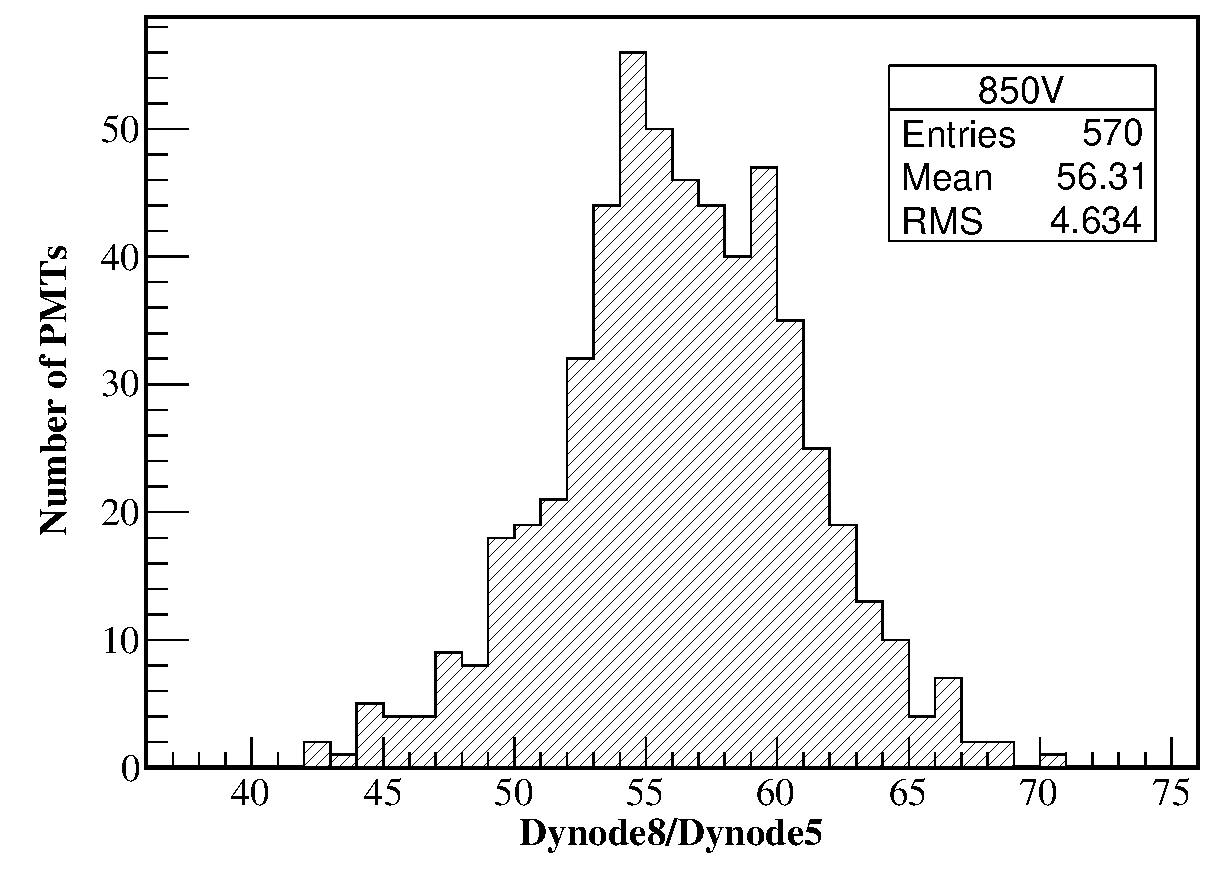
\includegraphics[width=0.49\textwidth]{chap/pmt_test/fig/dy58_distribution_850V.eps}
		\label{fig:pmt_test:dy58_distribution_850V}
	}
	\caption{Dy58比值的测试结果}
	\label{fig:pmt_test:dy58_results}
\end{figure}
根据得到的增益特性曲线,我们可以计算出任何工作电压下R4443的Dy58比值,图\ref{fig:pmt_test:dy58_distribution_850V}给出了\SI{850}{V}使所有管子的Dy58比值分布。

此次测试中,部分被测的PMT最终被挑选出来并安装到PSD上,它们经历了细致的宇宙线刻度测试(详见第\ref{ch:cosmicray_calibration}章)。
为了验证上述使用LED进行的Dy58比值测试的准确性,我们将这部分管子的LED测试结果和宇宙线刻度结果进行了比较,结果如图\ref{fig:pmt_test:dy58_ledvscm}所示。
\begin{figure}[htbp]
	\centering
	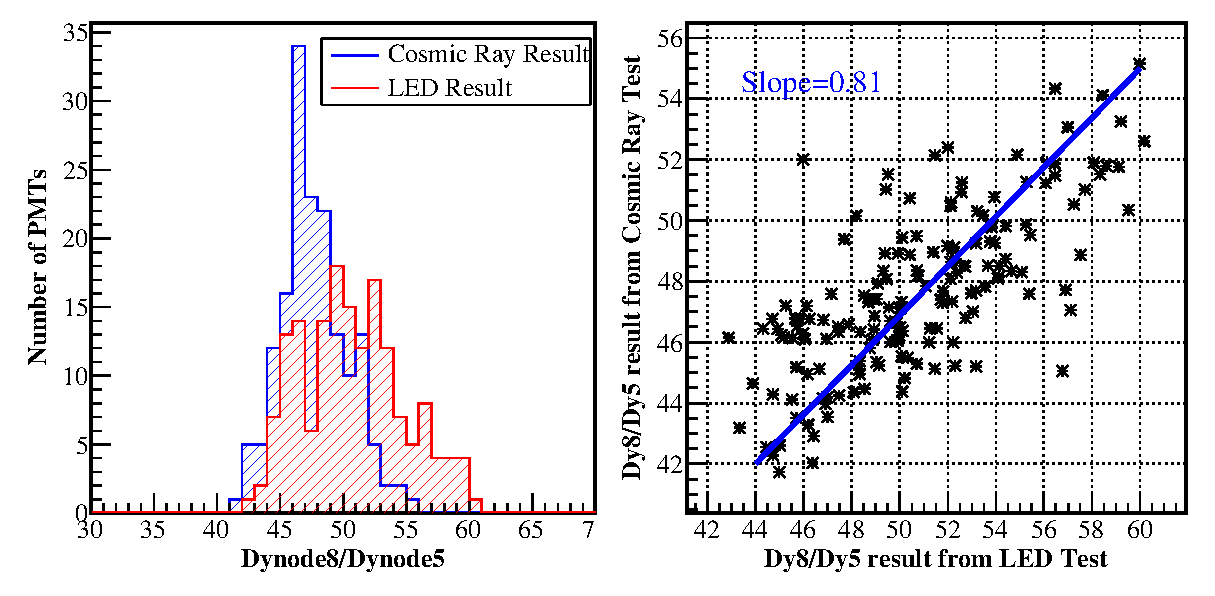
\includegraphics[width=0.95\textwidth]{chap/pmt_test/fig/dy58_ledvscm.eps}
	\caption{本次测试得到的Dy58比值与宇宙线测试得到的Dy58比值的比较}
	\label{fig:pmt_test:dy58_ledvscm}
\end{figure}
可以看到,宇宙线测试结果相对LED测试结果整体偏小,且分布较窄。
我们认为这些差异主要是入射光在光阴极上的分布不同引起的:LED测试时,入射光脉冲由光纤引出,光斑较小且只能照射PMT光阴极上某个固定点,而宇宙线测试时入射光是分布到整个光阴极面的。
即便如此,两个测试结果基本还是重合的,LED的测试结果仍然具有参考价值,我们使用的测试方法有效。

\subsection{光阴极均匀性的测量}
\label{sec:pmt_test:cathode_scanning}
由于光纤导出的光斑直径不到\SI{1}{mm},上述测试得到的结果严格来讲只是R4443光阴极中心处的性能参数。
实际使用中,R4443光阴极的大部分是被入射光覆盖的(大小取决于单元条端面与R4443端面的接触面积),因此其性能参数是所有光阴极位置点累计的结果。
如果光电倍增管的光阴极均匀性足够好,我们就能使用单个位置点得到的参数来代表整个管子的性能。
因此,我们也对部分被测R4443的光阴极进行了位置扫描,以考察单点测试结果的有效性。

R4443最小的有效光阴极面积为\SI{10}{mm}。
利用PMT批量测试平台的光阴极扫描功能,我们在竖直和水平方向上每隔\SI{1}{mm}对待测管子的相对增益进行了测量,图\ref{fig:pmt_test:cathode_uniformity}给出了一个示例结果。
\begin{figure}[htbp]
	\centering
	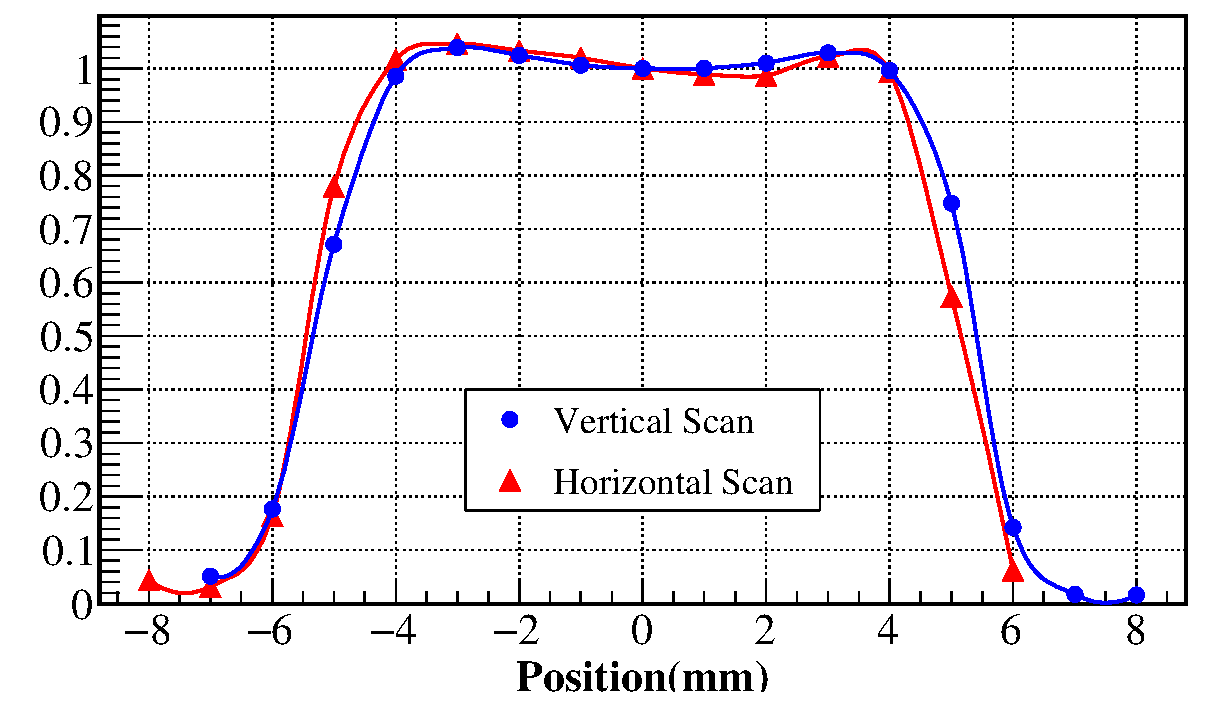
\includegraphics[width=0.65\textwidth]{chap/pmt_test/fig/cathode_uniformity.eps}
	\caption{R4443典型的光阴极均匀性}
	\label{fig:pmt_test:cathode_uniformity}
\end{figure}
可以看到,R4443光阴极中心区域的响应略小于边缘处,而在超过其有效面积后迅速减小到零。
为了对管子的非均匀性进行评估,我们以光阴极直径\SI{9}{mm}范围内的测量均值为中心值,计算出该范围内所有测量值相对中心值的最大偏差。
图\ref{fig:pmt_test:cathode_uniformity_distribution}给出了所有被测管子的最大偏差累积在一起的分布图。
对于PSD的PMT筛选来说(详见第\ref{ch:construction}章),$\pm\SI{10}{\percent}$的最大偏差是可以接受的,
从图\ref{fig:pmt_test:cathode_uniformity_distribution}可以看到,\SI{75}{\percent}管子的光阴极非均匀性都在这个区间内,因此我们的测试结果可以直接使用。

\begin{figure}[htbp]
	\centering
	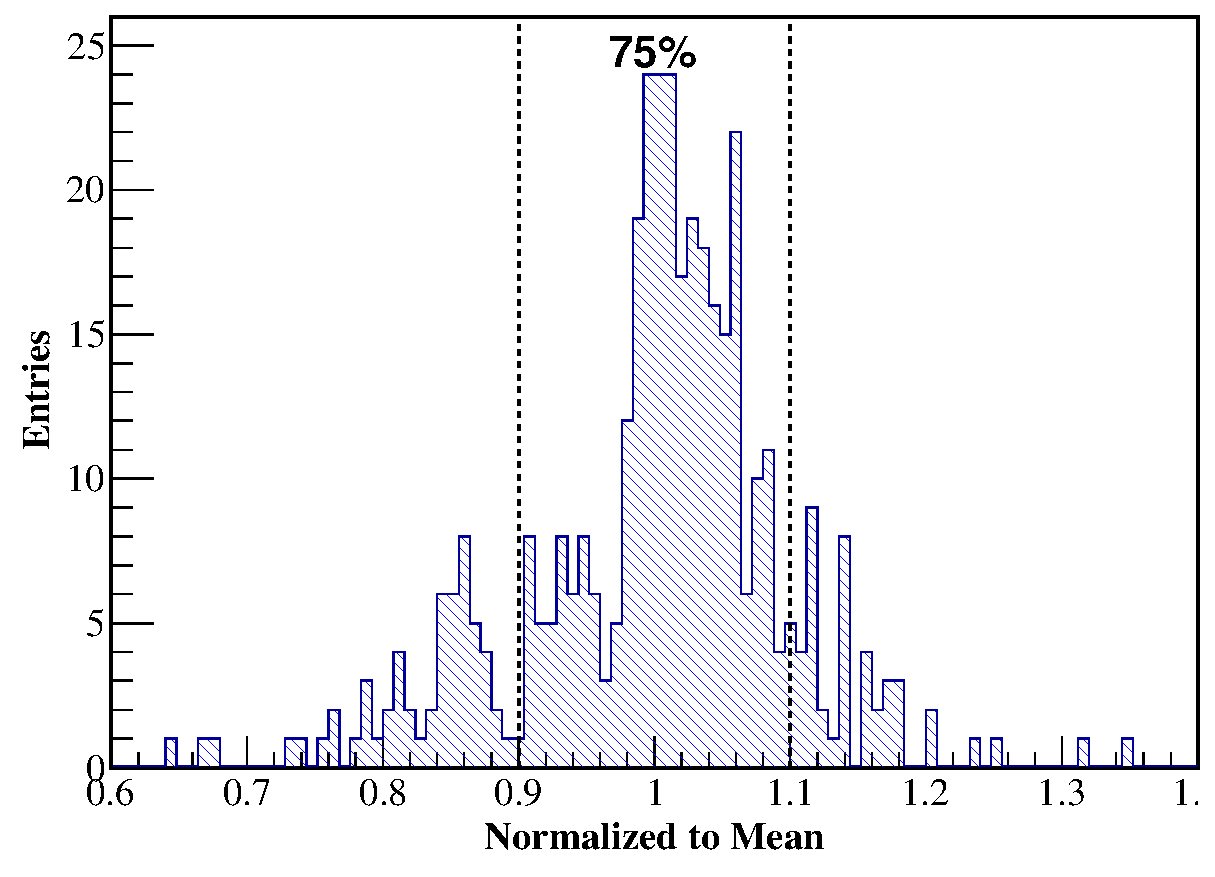
\includegraphics[width=0.65\textwidth]{chap/pmt_test/fig/cathode_uniformity_distribution.eps}
	\caption{R4443的光阴极均匀性分布}
	\label{fig:pmt_test:cathode_uniformity_distribution}
\end{figure}

\section{PMT批量测试平台在测试中的长期稳定性}
\label{sec:pmt_test:testbench_performance}

\begin{figure}[htbp]
	\centering
	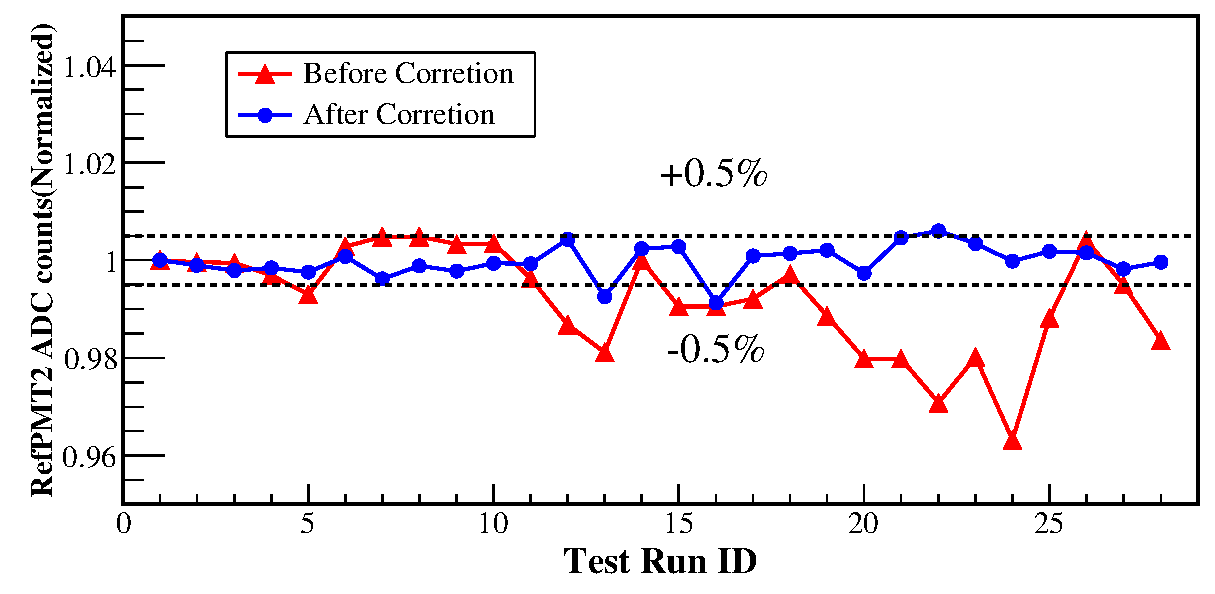
\includegraphics[width=0.65\textwidth]{chap/pmt_test/fig/led_stability.eps}
	\caption{LED光源的长期稳定性}
	\label{fig:pmt_test:led_stability}
\end{figure}

\begin{figure}[htbp]
	\centering
	\subfloat[][相对增益测试的稳定性]{
		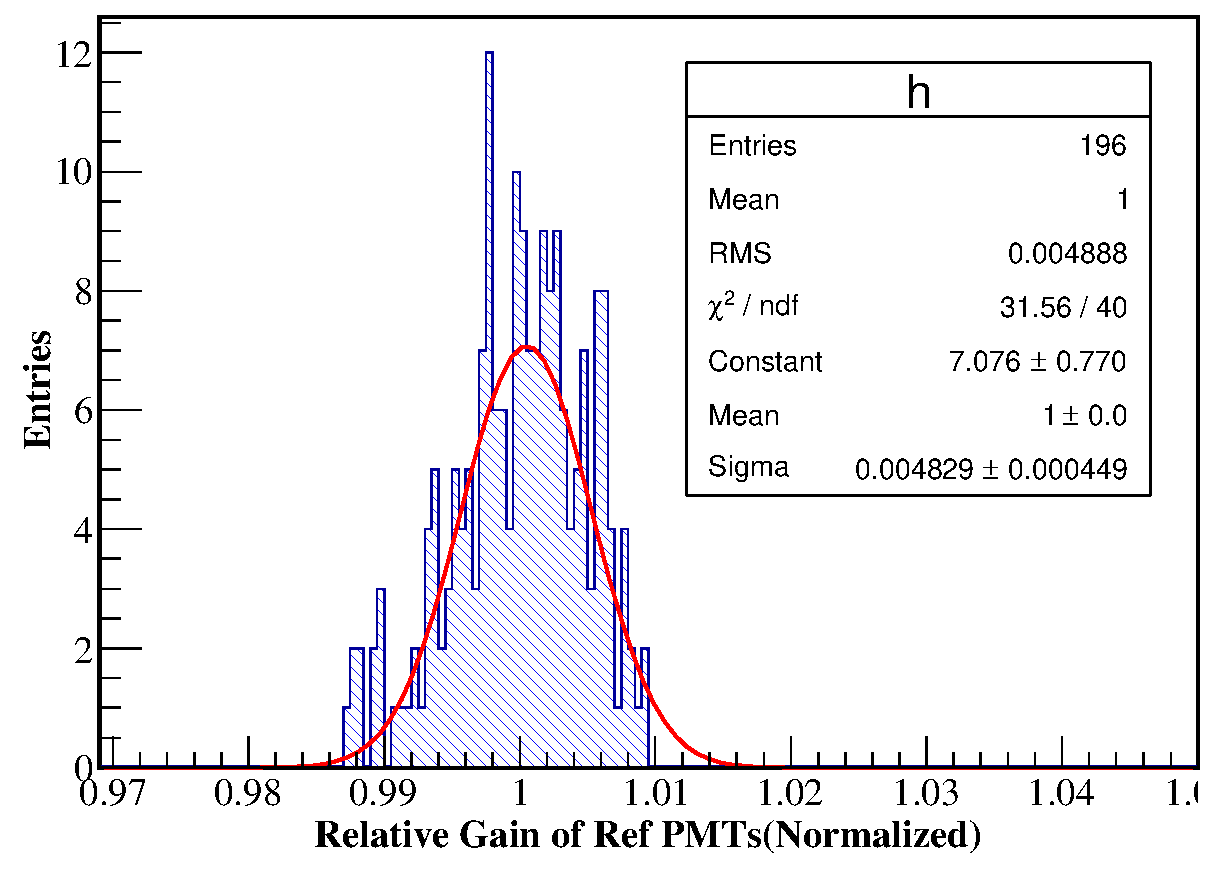
\includegraphics[width=0.48\textwidth]{chap/pmt_test/fig/ref_gain_stability.eps}
		\label{fig:pmt_test:ref_gain_stability}
	}
	\subfloat[][Dy58比值测试的稳定性]{
		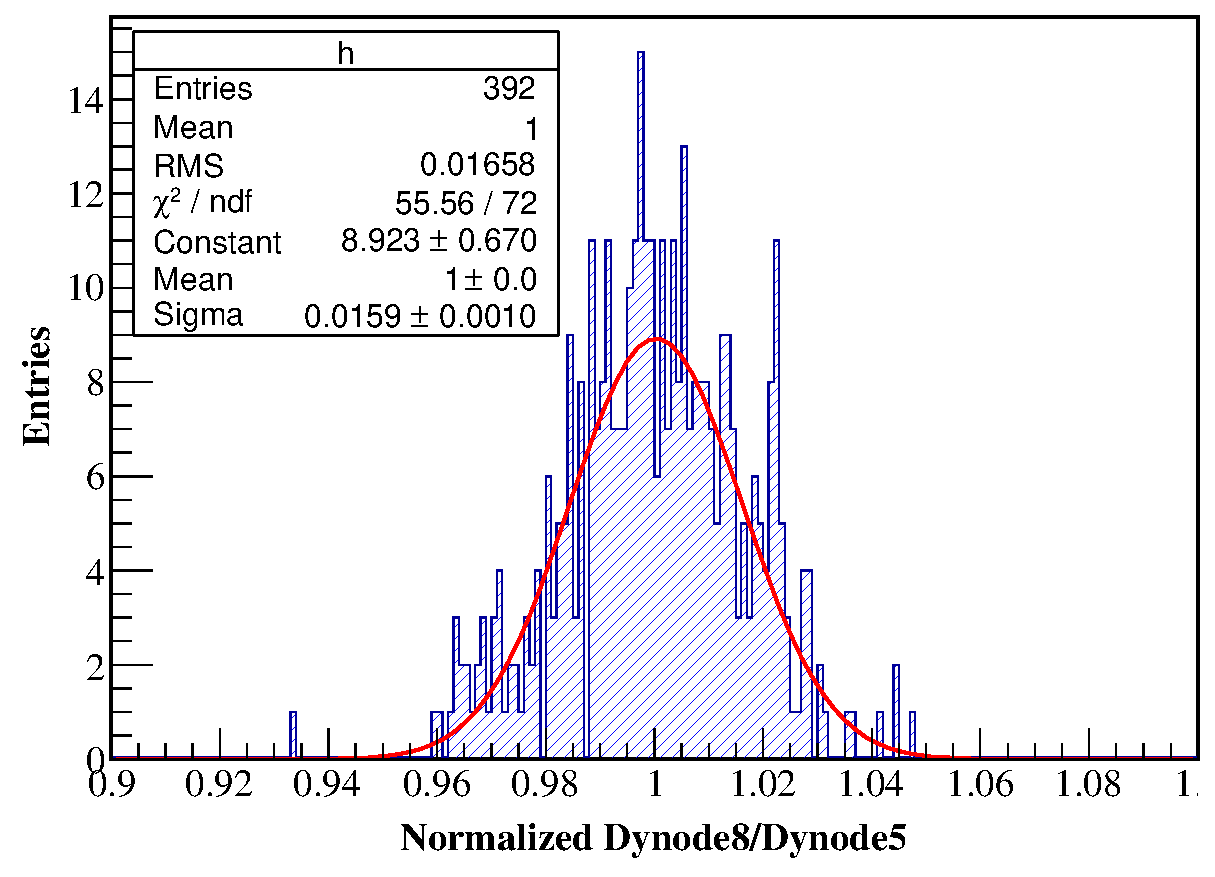
\includegraphics[width=0.48\textwidth]{chap/pmt_test/fig/ref_dy58_stability.eps}
		\label{fig:pmt_test:ref_dy58_stability}
	}
	\caption{PMT测试批量测试平台的性能稳定性}
	\label{fig:ref_stability}
\end{figure}
